% Generic (arXiv / readable) Supporting Information, built as its own file.
% Main text: paper_draft.tex. ACS build of the same pair: paper_jctc{,_si}.tex.
% Cross-document labels travel through xr-hyper, which reads paper_draft.aux, so both must be
% built after each other before every number settles. Compile: `make paper`.
\documentclass[11pt]{article}
\usepackage[utf8]{inputenc}
\usepackage[T1]{fontenc}
\usepackage[margin=1in]{geometry}
\usepackage{amsmath,amssymb,amsthm}
\usepackage{graphicx}
\usepackage{booktabs}
\usepackage{verbatim}
\usepackage[numbers,sort&compress]{natbib}
\usepackage{xr-hyper}
\usepackage[hidelinks]{hyperref}
\externaldocument{paper_draft}
\usepackage{xcolor}
\usepackage{enumitem}
\graphicspath{{../figs/}}

\theoremstyle{plain}
\newtheorem{theorem}{Theorem}
\theoremstyle{remark}
\newtheorem*{remark}{Remark}

\DeclareMathOperator{\Var}{Var}
\newcommand{\dF}{\Delta F}
\newcommand{\dFh}{\widehat{\Delta F}}
\newcommand{\ddG}{\Delta\Delta G}

\title{\bf Supporting Information for:\\
What Cycle Closure Can and Cannot See in a Relative Binding Free Energy Network}
\author{Nikita L. Polomoshnov\\
\small Faculty of Bioengineering and Bioinformatics, Lomonosov Moscow State University, Moscow, Russia\\
\small Institute of Biomedical Chemistry (IBMC), Moscow, Russia\\
\small \texttt{nikitapol@fbb.msu.ru}}
\date{\today}

\begin{document}
\maketitle

% S-prefixed pages, floats, sections and theorems, so nothing here collides with the main text.
\renewcommand{\thepage}{S\arabic{page}}
\renewcommand{\thefigure}{S\arabic{figure}}
\renewcommand{\thetable}{S\arabic{table}}
\renewcommand{\thesection}{S\arabic{section}}
\renewcommand{\thetheorem}{S\arabic{theorem}}
\setcounter{page}{1}

\section*{Supporting Information}

\paragraph{Reproducibility.} The analysis code released with this work regenerates every figure
in this article, each from a single command, and it emits the per-system tables reported here
from the same run that draws the corresponding figure, so the two cannot drift apart. This covers
the quality-control results (Figures~\ref{fig:L} and~\ref{fig:Lval} of the main text and
Figures~\ref{fig:Stab}, \ref{fig:OOS} and~\ref{fig:Self} here), the observability map of
Figure~\ref{fig:Lev}, the fixed-cutoff comparison of Figure~\ref{fig:Cut}, the $\sigma$-profile
sweeps of Figures~\ref{fig:P4} and~\ref{fig:P4b}, the autocorrelation panel of
Figure~\ref{fig:gsweep}, the curated-label grounding of Figure~\ref{fig:Ground} and
Table~\ref{tab:ground}, the label-noise floor of Figure~\ref{fig:Noise}, and the cross-release
split of Figure~\ref{fig:Release}. The constants appearing in the theorems and the invariants of the
cycle-closure test are additionally asserted as unit tests that run in the same environment.
Every input is public: the alchemtest BACE1 and benzene sets, the OpenFF
protein--ligand benchmark, ChEMBL~\citep{zdrazil2024chembl}, and the OpenFE
IndustryBenchmarks2024 replicate set~\citep{baumann2025industrybenchmarks}. Recalibration
baselines use temperature scaling~\citep{guo2017calibration} and isotonic
regression~\citep{zadrozny2002isotonic}.

\paragraph{BACE1 per-window overlap values (Figure~\ref{fig:A}).} Figure~\ref{fig:A} reports
that naive $1/I$ overstates the bootstrap se by $2$--$12\times$ on the $19$ real BACE1
adjacent-$\lambda$ BAR windows (mean $6.07$, $[2.78,12.01]$), the worst overstatement occurring at high
overlap, consistent with the controlled panel (invariant \#1, main text). These $19$ rows are the
windows of one $\lambda$ schedule, taken from the complex leg of the alchemtest AMBER
\texttt{load\_bace\_example} relative-binding calculation across its decharge, recharge and van
der Waals legs; each is a two-state BAR estimate between neighbouring $\lambda$ values, so the set
tests the closed-form variance against a decorrelated bootstrap on real molecular-dynamics works,
and it does not test $19$ separate binding free energies or reach beyond the high-overlap band this
schedule occupies. Table~\ref{tab:bace1}
lists the $(\lambda_i,\lambda_j)$ window labels, per-window overlap $4\langle p(1-p)\rangle$,
and both ratios for all $19$, emitted verbatim by the released analysis code, $\lambda$ labels
included, so the $\lambda$ pairing is re-derivable from it (seed $20260629$; both sandwich inputs
and the bootstrap truth subsampled to the statistical inefficiency $g$ before $B$ is formed,
Section~\ref{sec:bar}; numerically identical to the binding rows of the corresponding panel).
Every window sits at overlap $\geq0.84$ (mean $0.93$); the worst naive/bootstrap ratio ($12.01\times$)
occurs at the single highest-overlap window ($4\langle p(1-p)\rangle=0.992$), and the best (least
overstated, $2.78\times$) occurs at the lowest-overlap window in the set ($0.846$), the same
high-overlap-is-worst regime as the controlled sweep of Figure~\ref{fig:Afoils} rather than a property
of the particular windows sampled. The trend across the full $19$-window set is not confined to
the extremes: the Spearman rank correlation between overlap and the
naive/bootstrap ratio is $\rho=0.84$ ($n=19$, computed from Table~\ref{tab:bace1}), so the
relationship holds within the narrow $[0.846,0.992]$ overlap band, not just at its endpoints.

\begin{table}[t]\centering
\caption{\textbf{Per-window overlap on the $19$ real BACE1 adjacent-$\lambda$ BAR windows.}
$\lambda_i,\lambda_j$
are the BAR window endpoints; $4\langle p(1-p)\rangle$ is the normalized BAR overlap;
sandwich/boot and naive/boot are the reported-se/bootstrap-se ratios for the sandwich $B/I^2$
and the naive $1/I$, respectively, against a decorrelated-bootstrap reference standard error.
Rows are sorted by overlap, ascending; repeated $(\lambda_i,\lambda_j)$ pairs are distinct
windows from BACE1's decharge, recharge, and van der Waals alchemical legs, which share a
common $\lambda$ schedule.}
\label{tab:bace1}
\small
\begin{tabular}{@{}rrrrr@{}}
\toprule
$\lambda_i$ & $\lambda_j$ & $4\langle p(1-p)\rangle$ & sandwich/boot & naive/boot \\
\midrule
$0.437$ & $0.563$ & $0.846$ & $0.992$ & $2.780$ \\
$0.316$ & $0.437$ & $0.858$ & $1.001$ & $3.020$ \\
$0.206$ & $0.316$ & $0.876$ & $0.967$ & $4.377$ \\
$0.750$ & $1.000$ & $0.884$ & $0.956$ & $3.315$ \\
$0.563$ & $0.684$ & $0.909$ & $1.041$ & $3.451$ \\
$0.500$ & $0.750$ & $0.917$ & $0.971$ & $3.618$ \\
$0.684$ & $0.794$ & $0.921$ & $0.997$ & $3.581$ \\
$0.250$ & $0.500$ & $0.927$ & $1.017$ & $3.860$ \\
$0.000$ & $0.250$ & $0.928$ & $0.967$ & $3.678$ \\
$0.500$ & $0.750$ & $0.943$ & $1.018$ & $9.823$ \\
$0.794$ & $0.885$ & $0.943$ & $0.981$ & $4.165$ \\
$0.000$ & $0.250$ & $0.948$ & $0.986$ & $9.360$ \\
$0.115$ & $0.206$ & $0.949$ & $1.005$ & $6.414$ \\
$0.250$ & $0.500$ & $0.967$ & $1.004$ & $9.116$ \\
$0.750$ & $1.000$ & $0.968$ & $1.052$ & $9.901$ \\
$0.885$ & $0.952$ & $0.969$ & $0.995$ & $5.670$ \\
$0.952$ & $1.000$ & $0.983$ & $1.064$ & $8.193$ \\
$0.048$ & $0.115$ & $0.984$ & $1.066$ & $8.960$ \\
$0.000$ & $0.048$ & $0.992$ & $1.007$ & $12.007$ \\
\bottomrule
\end{tabular}
\end{table}

\paragraph{Autocorrelation robustness: raw $n$ vs $n_{\mathrm{eff}}=n/g$ (Figure~\ref{fig:gsweep}).}
The sandwich $B=n_f\Var_f[p]+n_r\Var_r[p]$ (Theorem~\ref{thm:sand}) assumes independent samples,
whereas real molecular-dynamics works are autocorrelated. On the $19$ real BACE1
adjacent-$\lambda$ BAR windows
of Figure~\ref{fig:A} (no new molecular dynamics), the sandwich se is recomputed at the raw sample count and again
after decorrelating each leg to its statistical inefficiency $g$~\citep{shirts2008mbar}
(geometric-mean $\bar g=1.48$, range $[1.15,2.16]$; median count $n{=}500\to349$). Against the
correlation-aware truth (the decorrelated bootstrap standard deviation, the same reference as
Figure~\ref{fig:A}),
the $n_{\mathrm{eff}}$ sandwich is calibrated, at a reported/truth ratio of $1.00$ $[0.93,1.07]$,
reproducing Figure~\ref{fig:A}. The raw-$n$ sandwich is overconfident by $0.83\times$
$[0.67,0.97]$, matching the $1/\sqrt{\bar g}=0.82$ autocorrelation prediction. The sandwich also tracks its
own matched (raw) bootstrap ($1.00$, $[0.92,1.05]$): the closed form is internally
consistent, and the only quantity that must be right is the effective sample count, which the paper
decorrelates to $g$ throughout (Section~\ref{sec:bar}, main text). The calibration verdict is
therefore robust to autocorrelation once $n_{\mathrm{eff}}$ is used, as it is in every real-data
panel.

\begin{figure}[t]\centering
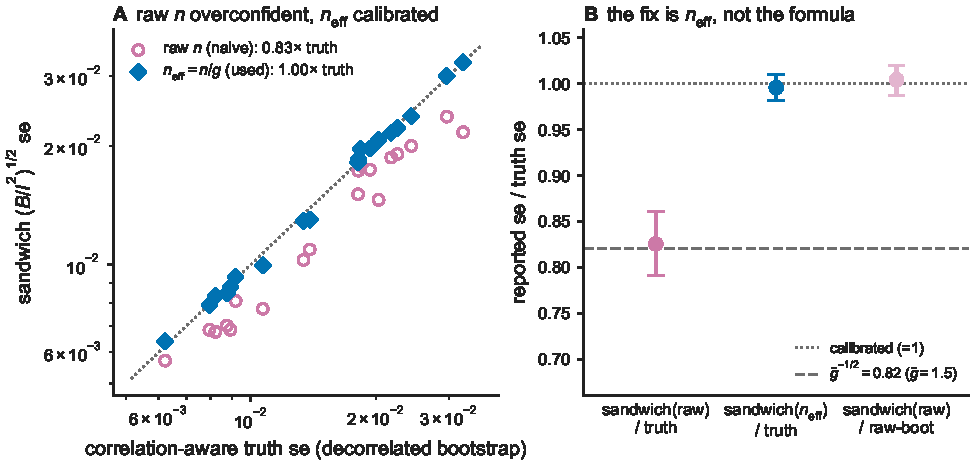
\includegraphics[width=\textwidth]{figAC_gsweep.pdf}
\caption{\textbf{Sandwich standard error at the raw sample count versus at the effective
sample count $n_{\mathrm{eff}}=n/g$, on the real BACE1 $\lambda$ windows.} (A) Sandwich standard error at
$n_{\mathrm{eff}}$ and at raw $n$, plotted against the correlation-aware (decorrelated
bootstrap) reference standard error, with the $y{=}x$ line. (B) Aggregate ratio of sandwich
standard error to the reference, at $n_{\mathrm{eff}}$, at raw $n$, and of the sandwich to
its own raw-$n$-matched bootstrap, with bootstrap confidence intervals; the
$1/\sqrt{\bar g}$ autocorrelation prediction is marked.}
\label{fig:gsweep}
\end{figure}

\paragraph{The learned-variance comparison (Figure~\ref{fig:Afoils}).} Figure~\ref{fig:Afoils} is
the controlled overlap sweep behind the comparison the main text states: the sandwich $B/I^2$
coincides with \texttt{pymbar}-MBAR and with Monte-Carlo truth across the range, while a fair
learned mean--variance head, given the same overlap information the closed form uses, is
overconfident at a realistic label budget and remains so at a twenty-fold larger one. Two
restrictions travel with the figure. The head is trained and measured here, but its use as a
comparison bar downstream is a counterfactual: no deployed or published pipeline is known to feed a
learned per-edge $\sigma$ into a network consistency check, and the arms built from its measured
miscalibration in the quality-control and stopping experiments are comparison models rather than
estimators run in those experiments. And the overconfidence is a property of the per-edge
parameterisation rather than of learning from labels, since on the identical labels pooling
single-label edges by overlap recovers the sandwich to $\sim$6\% at $4000$ edges (below).

\begin{figure}[t]\centering
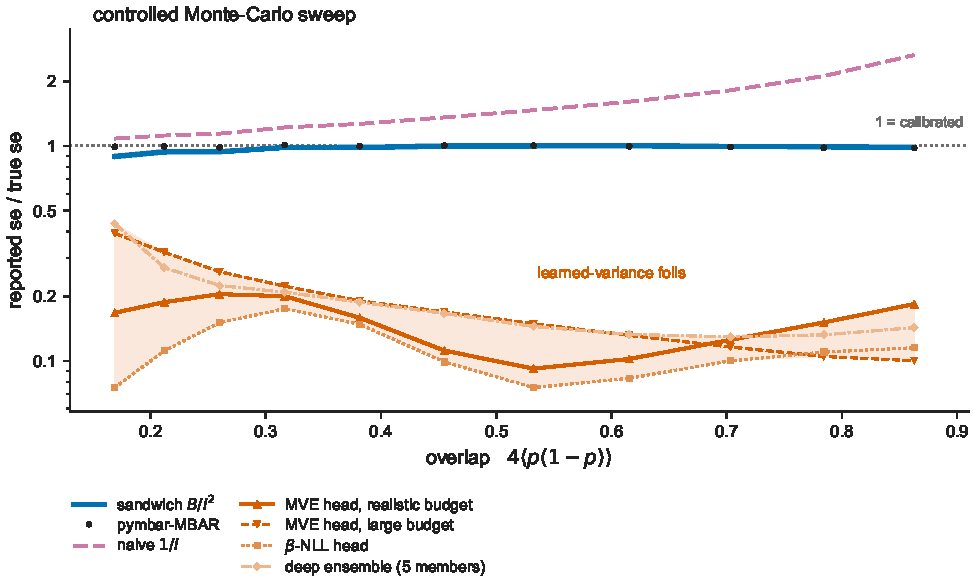
\includegraphics[width=\textwidth]{figA_learned_foils.pdf}
\caption{\textbf{Reported standard error against the true standard error over a controlled overlap
sweep.} Reported standard error divided by the true standard error, versus work-distribution
overlap, for the sandwich $B/I^2$, \texttt{pymbar}-MBAR, the naive information-equality
plug-in $1/I$, a learned mean--variance (MVE) head at a realistic and at a large training
budget, a $\beta$-NLL head, and a $5$-member deep ensemble, in a controlled Monte-Carlo
sweep.}
\label{fig:Afoils}
\end{figure}

\paragraph{Corrected learned-variance foils and the data-efficiency floor (Figure~\ref{fig:Afoils}).}
Neither correction restores the head's calibration at a realistic budget. A head trained on the
$\beta$-weighted negative log-likelihood ($\beta$-NLL)~\citep{seitzer2022pitfalls}
($\beta{=}0.5$, the standard objective correction) does not recover calibration (se ${\approx}0.11\times$, slightly worse than plain NLL's
$0.15\times$), and at this training seed a $5$-member deep
ensemble~\citep{lakshminarayanan2017ensembles} reaches only the large-budget floor
(se ${\approx}0.20\times$, the same ${\approx}5\times$ overconfidence a $20\times$-larger-budget
plain head reaches).
The residual $\sim$5$\times$ overconfidence of the plain, oracle and $\beta$-NLL heads is
therefore a property of the per-edge parameterisation rather than of the label budget or of
the Gaussian-NLL objective. The conditional variance $se(\text{overlap})$ is identifiable from
single labels, and pooling single-label edges by overlap recovers the sandwich to $\sim$6\% at
$4000$ edges ($\sim$4\% at $40000$) on the same labels the heads were given. This bears on the
scope of the quality-control comparison. Placing a $6\%$ miscalibration on the frozen
scale grid of Figure~\ref{fig:P4b} gives seven flagged systems of $48$ against the published six, and
a $6\%$ over-estimate gives six; the test is unchanged. The collapse to $42$ of $48$ requires the
$5$--$11\times$ under-estimate the trained per-edge heads produce, so the contrast is scoped to
heads of that kind and is not evidence that a same-budget learned estimator must break the test.

\paragraph{Seed stability of the learned-variance foils (Figure~\ref{fig:Afoils}).}
These ratios are stable across independent training seeds for the plain and
$\beta$-NLL heads: over $5$ seeds the plain head spans $0.1229$--$0.2103\times$ (mean
$0.1537\times$) and the $\beta$-NLL head $0.1024$--$0.1256\times$ (mean $0.1147\times$), so their
overconfidence is a property of the estimator at this budget rather than of a single
initialization. The $5$-member ensemble is not stable: across the same $5$ seeds, each with a
disjoint $5$-network member block, it spans $0.1984$--$1.2200\times$ (mean $0.4198\times$, sd
$0.4481\times$), and one seed overestimates the true se by $22\%$, crossing perfect
calibration. Unlike the plain, oracle ($0.1941$--$0.2571\times$, mean $0.2101\times$), and
$\beta$-NLL heads, whose overconfidence is robust across independent retrains, the ensemble is
unreliable in both directions at this budget.

\paragraph{Synthetic decomposition (illustration).} In a controlled one-dimensional problem whose
generative structure is known, the decomposed interval is up to $2.2\times$ sharper than a
split-conformal interval ($2.0\times$ sharper than conformalized quantile
regression~\citep{romano2019cqr}) at equal
coverage, with better conditional calibration. The problem illustrates the mechanism; the evidence
on real data is Figure~\ref{fig:Breal}.

\paragraph{Edge weighting (Figure~\ref{fig:C}).} The acquisition policy outperforms random
selection by a factor of $2.2$. Changing the edge weighting from naive to sandwich changes
calls-to-top-$k$ by a factor of $0.98$ $[0.93,1.03]$ ($24$-seed bootstrap confidence interval),
which is the Gauss--Markov ceiling on the choice of weights.

\begin{figure}[t]\centering
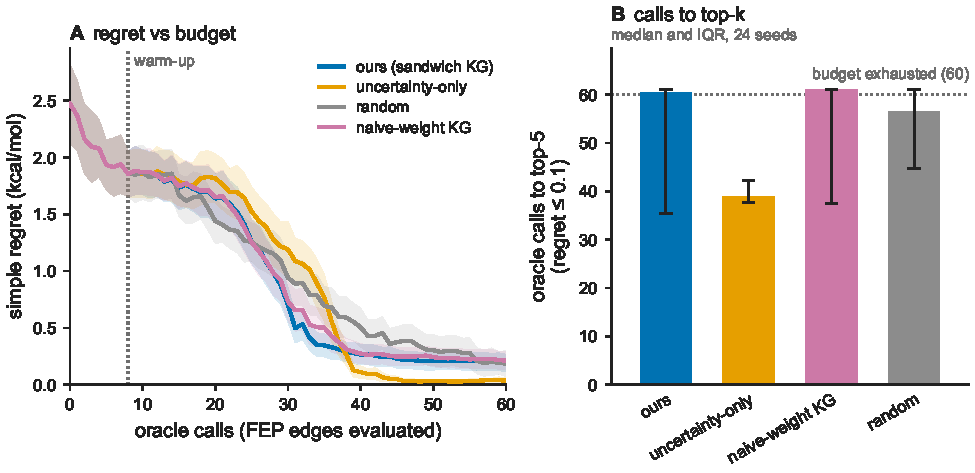
\includegraphics[width=\textwidth]{figC_active_learning.pdf}
\caption{\textbf{Simulated active-learning acquisition policies.} (A) Simple regret versus
oracle calls (simulated FEP edges evaluated), for a sandwich-weighted knowledge-gradient
policy~\citep{frazier2008kg}, implemented as in~\citet{balandat2020botorch}
and~\citet{gardner2018gpytorch},
a naive-weighted knowledge-gradient policy, an uncertainty-only policy, and random
selection, averaged over $24$ seeds with $95\%$ confidence bands. (B) Median oracle calls to
reach the top-$k$ candidates (regret at or below tolerance), with interquartile-range error
bars, for the same four policies.}
\label{fig:C}
\end{figure}

\paragraph{The Fisher--resistance correspondence.} The theorem below establishes what the
per-edge bar buys the decision layer: with the inverse sandwich variances as conductances, the
Gaussian posterior precision of the node potentials is a weighted Laplacian, contrast variance is
effective resistance, acquisition updates are $O(1)$, and the knowledge gradient is exactly zero on
gauge directions. It is stated here because what the article measures downstream of it is that the
weight \emph{value} is second-order for ranking: in a connected graph
the generalized-least-squares contrast mean is unbiased for any positive conductances, so by
Gauss--Markov the choice of weights cannot improve a ranking (Table~\ref{tab:audit} below). The
theorem's content is accordingly the gauge-invariance, which is structural and holds for any
positive conductances, and which the simulation of Figure~\ref{fig:D} exercises.

\begin{theorem}[Fisher--resistance correspondence]\label{thm:fr}
For relative measurements $y_e=(\varphi_j-\varphi_i)+\varepsilon_e$,
$\varepsilon_e\sim\mathcal N(0,V_e^{\mathrm{true}})$ with $V_e^{\mathrm{true}}=B_e/I_e^2$, the
Gaussian posterior precision of
the node potentials is the weighted Laplacian $L=\sum_e w_e(e_i-e_j)(e_i-e_j)^\top$ with
conductances $w_e=1/V_e^{\mathrm{true}}=I_e^2/B_e$. Contrast variance equals effective
resistance~\citep{klein1993resistance}, a single edge recovers $V_e^{\mathrm{true}}$,
Sherman--Morrison gives
$O(1)$ acquisition updates, and $\ker L\supseteq\mathrm{span}\{\mathbf 1\}$, so the knowledge
gradient (KG)~\citep{frazier2008kg} is exactly zero on gauge/redundant directions: the acquisition is
automatically gauge-invariant.
\end{theorem}
The edge weights are the inverse sandwich variances, the readout of Section~\ref{sec:bar}
entering the decision layer; the acquisition model identifies the reported variance with the true
one ($c_e=1$), an assumption the replicate validation of Section~\ref{sec:bar} tests rather than
one this section adds. The gauge-zero property is structural: KG$=0$ on gauge directions
follows from the kernel inclusion alone, so it does not depend on the weight value, and by
Gauss--Markov the value does not improve ranking (Table~\ref{tab:audit} below). For a \emph{connected}
network the inclusion is an equality, $\ker L=\mathrm{span}\{\mathbf 1\}$, for any positive
conductances, and the overall additive offset is then the only unidentifiable direction; a network
with $k$ components has a $k$-dimensional kernel, one offset per component. The
Laplacian-precision and resistance-distance machinery is classical generalized least squares (GLS)
on graphs and the resistance distance of \citet{klein1993resistance}; what is specific here is the
sandwich precision $I_e^2/B_e$ as the conductance, in place of raw overlap, and the automatic
gauge-invariance of the acquisition.

\paragraph{Gauge-aware acquisition (Figure~\ref{fig:D}).} The Fisher--resistance Laplacian
(Theorem~\ref{thm:fr}) makes the knowledge gradient exactly zero on gauge (all-ones) contrasts. A
controlled simulation gives $\mathrm{KG}=10^{-21}$ on the all-ones gauge contrast, an exact zero,
and the identifiability statement behind it transfers structurally to multi-target networks. A
gauge-unaware acquisition spends budget resolving a decision-irrelevant cross-cluster offset,
reaching the within-target top-$k$ at regret $0.27$ where the gauge-aware one reaches $0.01$.

\begin{figure}[t]\centering
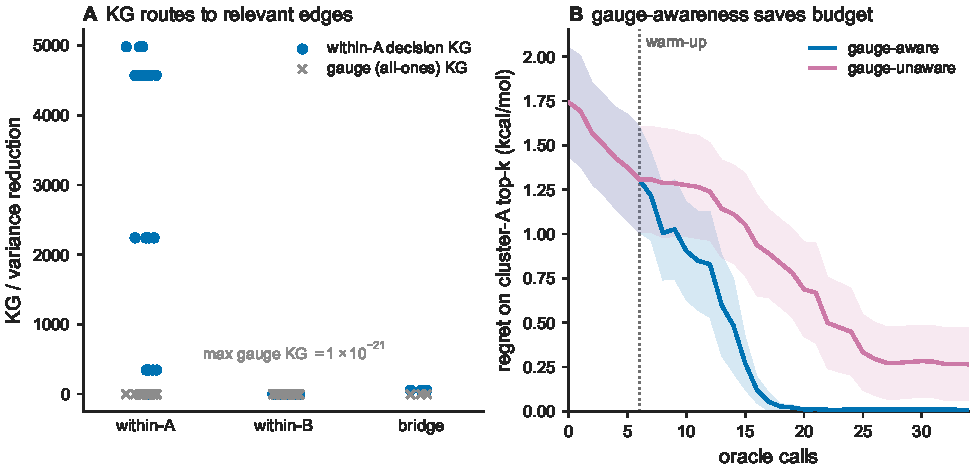
\includegraphics[width=\textwidth]{figD_gauge_identifiability.pdf}
\caption{\textbf{Knowledge-gradient score on gauge and decision-relevant contrasts
(simulation).} (A) Knowledge gradient for the within-cluster decision contrast and for the
gauge (all-ones) contrast, by edge type (within-cluster-A, within-cluster-B, bridge). (B)
Regret on the cluster-A top-$k$ candidates versus oracle calls, for a gauge-aware and a
gauge-unaware acquisition policy, averaged over seeds with $95\%$ confidence bands.}
\label{fig:D}
\end{figure}


\paragraph{Structural context of the flagged systems (Figure~\ref{fig:qcstruct}).}
Two of the systems the closure test flags (Figure~\ref{fig:L}) carry an
independently-documented hard structural feature, read here directly from public co-crystal
structures. In BACE1 (PDB 4DJW) the catalytic aspartic-acid dyad hydrogen-bonds the inhibitor
(Asp93 and Asp289, both $2.7$\,\AA); the protonation state of an aspartic-protease dyad is a
recognized source of free-energy error. In BRD4 BD1 (PDB 3MXF, in complex with
JQ1~\citep{filippakopoulos2010bet}) the acetyl-lysine pocket packs $16$ crystallographic waters
within $4.5$\,\AA\ of the ligand ($8$ within $3.5$\,\AA) around the recognition asparagine Asn140
($3.1$\,\AA); this conserved water network is the known BRD4 free-energy challenge~\citep{aldeghi2016binding}.
The other flags carry analogous a-priori difficulties: \texttt{faah} (covalent serine hydrolase,
large acyl channel), \texttt{cdk8} and \texttt{p38} (large scaffold and R-group changes), and
\texttt{hif2a} (a buried polar cavity). The context is retrospective and structural rather than a per-edge causal claim: cycle closure is
edge-level and blind to node-consistent bias (main text). It establishes only that the flagged set
coincides with the features a domain expert would identify a priori. In
Figure~\ref{fig:qcstruct} the colours annotate structural objects rather than methods.


\begin{figure}[t]\centering
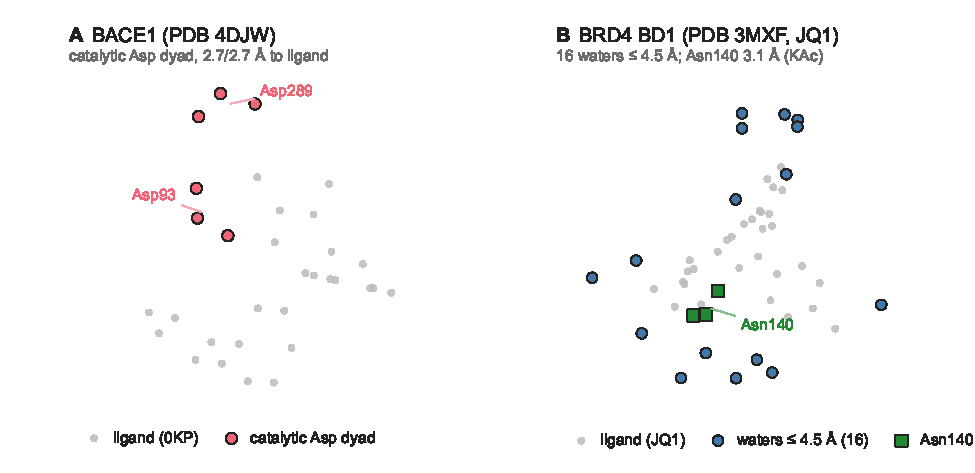
\includegraphics[width=\textwidth]{figQC_structures.pdf}
\caption{\textbf{Structural context of two flagged systems, from public co-crystal
structures.} Heavy-atom coordinates.
(A) BACE1 (PDB 4DJW): the catalytic aspartic-acid dyad (Asp93/Asp289, red circles) and the bound
inhibitor (grey). (B) BRD4 BD1 (PDB 3MXF, in complex with JQ1): crystallographic waters within
$4.5$\,\AA\ of the ligand (blue circles), the recognition residue Asn140 (green squares), and
the ligand (grey).}
\label{fig:qcstruct}
\end{figure}

\paragraph{Per-edge observability map and predictive falsifier (Figure~\ref{fig:Lev}).} The
estimation--detection conservation law (Theorem~\ref{thm:cons}) certifies $\sum_e h_e=\mathrm{dof}$
to machine precision (maximum deviation $1.78\times10^{-14}$) across the $48$ cyclic systems and
identifies $48$ structurally un-auditable bridge edges ($h_e=0$, one per system on average); a
pre-registered test of whether the curl-leverage also predicts the location of
reproducible systematic error, run on $934$ pooled edges over $45$ systems against the rule
confirmed if and only if $\rho>0$ and $p<0.05$ ($10^4$ within-system block permutations), is negative (studentized Spearman $\rho=-0.073$, $p=0.9571$), so only the structural certificate is claimed.

\paragraph{Per-system auditability (Table~\ref{tab:auditability}).} Theorem~\ref{thm:hodge} makes
a network's auditable fraction a property of its topology and its reported precisions alone, so it
can be tabulated for every benchmark system before any question of what that system's error turns
out to be. Table~\ref{tab:auditability} gives, per system, the ligand and edge counts, the number
of independent cycles $\nu$, the auditable fraction $\nu/E$, the bridge count, and the median
detectable shift over that system's auditable edges.
The auditable fraction is exactly $1-(N-c)/E$, for $N$ ligands, $E$ edges and $c$ connected
components, and so is small wherever a network is sparse: it
runs from $0.12$ to $0.46$ with a median of $0.31$, and no benchmark system exposes more than half
of its own error space to the test. The eight flagged systems span essentially that whole range,
from $0.12$ to $0.46$, rather than concentrating at the auditable end: a system is
flagged for the error it carries, not for how much of that error is in view. \texttt{brd4}, flagged on two of the three replicates, sits
at the bottom of the table with a single independent cycle: its reduced $\chi^2$ is a
one-degree-of-freedom statistic, which is the quantitative form of the caution
Section~\ref{sec:stability} places on it. Rows are ordered by auditable fraction, and the flag
marks are recomputed from the three replicates by the same code that draws
Figure~\ref{fig:Hodge}, not transcribed from the main text.

\paragraph{What was pre-registered.} Several arguments in this article turn on what was frozen
before the computation rather than chosen after it. The design file governing the decomposition
increment was committed to the article's repository before the commit that computes any of the
quantities it governs, and it is released with the analysis code; the Data and Software
Availability statement says where. It fixes three items and no others: H1, the visible fraction of
the measured error against experiment with its chance level and its success criterion; H2, the
influence-ranked repair race; and H3, the auditability map, which it labels descriptive and gives
neither threshold nor verdict. Both
success criteria are conjunctive, so a single conjunct firing is not a success. H1 is labelled a
quantification backed by an identity rather than a risky test, and says why: experimental
affinities are per-ligand, so $\Pi\varepsilon$ reduces to the closure residual and the visible
fraction is an identity, with only the comparison against the chance level at risk. The confound
the design cannot resolve is declared in it: experimental measurement error and the stereo-blind
affinity join are both per-ligand and therefore also gradient fields, so the design cannot separate
per-ligand force-field bias from per-ligand experimental or annotation error, and the conclusion it
licenses is the first of those and not the second. H2 is declared in the design file to be a second
look at data that had already produced one null, and its result carries that status.

The other pre-specified constants this article invokes are recorded in the released analysis code
and in the pre-registration for the experiment that fixed them, not in that file: the $|z|$-rule
conjunctive criterion, the curl-leverage falsifier rule, the fixed-cutoff head-to-head criterion,
the $1.0$ kcal/mol cutoff itself, the swept scale grid with its two frozen readouts, the per-edge
granularity of the self-calibrated null, and the close-the-loop criterion. Three of them live only
in code, and the paragraph below audits those three against the descriptions printed here.

\paragraph{Audit of the frozen criteria that live only in code.} Three criteria are recorded in the
analysis code and not in the design file, and each is audited here against the description printed
in this article. The
curl-leverage falsifier is confirmed if and only if $\rho>0$ with a within-system block-permutation
$p<0.05$ over $10^4$ permutations; the code implements that rule and the supplement prints it. The fixed-cutoff head-to-head requires the calibrated test's detection area to exceed
both baselines, implemented as a paired bootstrap of
$\mathrm{AUC}(A)-\max(\mathrm{AUC}(B),\mathrm{AUC}(C))$ with a win declared only when the point
difference is positive and the lower confidence bound excludes zero; the printed description
matches, and the tie follows from the $+0.140$ $[-0.008,0.316]$ against the stronger baseline. The
$|z|$-rule conjunctive criterion matches the code as printed here, requiring Stouffer $p<0.05$ and
a guided $\Delta$MUE above the $95$th percentile of its own random null in a majority of grounded
systems, and that is the upper tail because $\Delta$MUE is defined as
$\mathrm{MUE}(\text{full})-\mathrm{MUE}(\text{after})$, so an improvement is positive. Its frozen
file names the lower tail, ``below the 5th percentile'', which is the same event stated in the
opposite sign convention; the code's variable name follows the file rather than the statistic. No
result depends on the discrepancy. The frozen file is unaltered, and the description printed in
this article is the one the code implements.

\paragraph{The visible fraction is metric-dependent (Section~\ref{sec:hodge}).} The visible
fraction $f$, the share of the error against experiment lying in the auditable subspace
(Section~\ref{sec:hodge}), is a ratio of squared norms, so it depends on the metric those
norms are taken in, and the main text quotes it in the variance-weighted metric the closure
statistic itself uses. Three readings of the same four sub-networks are collected in
Table~\ref{tab:metrics}, each with its own chance level and with the range the fraction takes when
one edge is deleted at a time. The whitened reading takes both quantities in the variance-weighted
metric the closure statistic lives in, against $\mathrm{dof}/E$. The isotropic reading keeps that
fraction and measures it against $\mathrm{tr}(\Pi W)/\mathrm{tr}(W)$, the chance level an error
isotropic in kcal/mol would produce under the same projector; it gives the weakest margins, and it
is the reading the abstract and the main text quote. The unweighted reading recomputes the
projector itself in the unweighted metric, $\Pi=I-A(A^{\top}A)^{+}A^{\top}$ on the raw incidence
matrix $A$, so neither the fraction nor its chance level carries any variance weighting; there the
pooled fraction rises from $0.6\%$ to $5.45\%$. The worst single cell in the whole table is
\texttt{bace} under the isotropic reading with one edge deleted, at a factor of $1.36$ below its
chance level. Both the fraction and the chance level are recomputed on every deletion, since
deleting an edge moves the projector as well; \texttt{make figHodge} produces the table.
\texttt{cdk8}'s flag arises from a naming collision between two releases rather than from either
release's simulations (Section~\ref{sec:qc}), so the pooled figure is given both ways: $0.0060$ whitened and
$0.0545$ unweighted over the four systems, $0.0060$ and $0.0610$ with \texttt{cdk8} dropped, so the
whitened headline does not depend on it. Recomputing the ratio on medians rather than sums, which
removes any dependence on a few large residuals, gives $0.0034$, $0.0068$, $0.0052$ and $0.0015$,
the same order throughout; and \texttt{bace}, the one grounded system whose ligand set contains no
enantiomer pair collapsed by the stereo-blind affinity join, shows the effect as plainly as the
three that do. Every reading puts $f$ below its own chance
level; what changes is by how much, and the conclusion the main text draws is the weakest of them.

\begin{table}[tp]\centering
\caption{\textbf{The visible fraction under three metric conventions.} For each grounded system: edges $E$, independent cycles $\nu$, the auditable share of that system's error against experiment, the chance level it is measured against, their ratio, the range the fraction takes when one edge is deleted at a time, and the worst margin over those deletions with both the fraction and the chance level recomputed on each. \emph{Whitened} takes both in the variance-weighted metric the closure statistic lives in, against $\nu/E$. \emph{Isotropic} keeps that fraction and measures it against the chance level an error isotropic in kcal/mol would produce under the same projector, $\mathrm{tr}(\Pi W)/\mathrm{tr}(W)$. \emph{Unweighted} recomputes the projector in the unweighted metric, so neither the fraction nor its $\nu/E$ chance level carries any variance weighting. Every cell of every convention, and every single-edge deletion, sits below its own chance level; the weakest is \texttt{bace} isotropic under deletion. Pooled over the four systems the fraction is $0.0060$ whitened and $0.0545$ unweighted, and $0.0060$ and $0.0610$ with \texttt{cdk8} dropped. Produced by \texttt{make figHodge}.}
\label{tab:metrics}
\small
\begin{tabular}{@{}lrrlrrrlr@{}}
\toprule
system & $E$ & $\nu$ & metric & visible & chance & margin & leave-one-out & worst \\
\midrule
\texttt{cdk8} & $31$ & $9$ & whitened & $0.0065$ & $0.2903$ & $44.8\times$ & $[0.0034,0.0113]$ & $23.60\times$ \\
& & & isotropic, kcal/mol & $0.0065$ & $0.1273$ & $19.6\times$ & $[0.0034,0.0113]$ & $7.36\times$ \\
& & & unweighted & $0.0286$ & $0.2903$ & $10.2\times$ & $[0.0178,0.0324]$ & $8.22\times$ \\
\addlinespace[2pt]
\texttt{hif2a} & $59$ & $19$ & whitened & $0.0017$ & $0.3220$ & $187.2\times$ & $[0.0010,0.0029]$ & $106.60\times$ \\
& & & isotropic, kcal/mol & $0.0017$ & $0.0510$ & $29.6\times$ & $[0.0010,0.0029]$ & $13.21\times$ \\
& & & unweighted & $0.0172$ & $0.3220$ & $18.7\times$ & $[0.0127,0.0188]$ & $16.53\times$ \\
\addlinespace[2pt]
\texttt{p38} & $51$ & $18$ & whitened & $0.0086$ & $0.3529$ & $41.0\times$ & $[0.0033,0.0132]$ & $25.81\times$ \\
& & & isotropic, kcal/mol & $0.0086$ & $0.1240$ & $14.4\times$ & $[0.0033,0.0132]$ & $1.46\times$ \\
& & & unweighted & $0.1371$ & $0.3529$ & $2.6\times$ & $[0.0285,0.1499]$ & $2.31\times$ \\
\addlinespace[2pt]
\texttt{bace} & $26$ & $5$ & whitened & $0.0460$ & $0.1923$ & $4.2\times$ & $[0.0027,0.0628]$ & $2.55\times$ \\
& & & isotropic, kcal/mol & $0.0460$ & $0.0919$ & $2.0\times$ & $[0.0027,0.0628]$ & $1.36\times$ \\
& & & unweighted & $0.0564$ & $0.1923$ & $3.4\times$ & $[0.0033,0.0707]$ & $2.26\times$ \\
\addlinespace[2pt]
\bottomrule
\end{tabular}
\end{table}


The label source can also be changed. The measurement uses a stereo-blind, target-wide ChEMBL
search under the coverage rule, and the OpenFF protein--ligand benchmark of the downstream audit
below (Table~\ref{tab:audit}) carries curated
per-edge experimental $\ddG$ for three of the four systems (\texttt{bace} has none). Matching those
to the network by canonical SMILES recovers $57\%$, $98\%$ and $91\%$ of the curated edges for
\texttt{cdk8}, \texttt{hif2a} and \texttt{p38}. The matched sub-networks are much smaller than the
grounded ones and \texttt{p38}'s retains no cycle, so the check is weak, but where it can be run it
agrees: the visible fraction on curated labels is $0.0007$ for \texttt{cdk8} against a chance level
of $0.071$, and $0.0006$ for \texttt{hif2a} against $0.147$. Comparing those two figures against
what the ChEMBL labels give is only meaningful on identical edges. Against the full systems'
ChEMBL fractions, measured over $31$ and $59$ edges rather than over these $14$ and $34$, the
curated reading is the lower one; restricted to the same edges it is the higher one, $0.00071$ and
$0.00063$ against $0.00016$ and $0.00021$, by factors of $4.4$ and $2.9$. The direction on
identical edges is the one the decomposition predicts. A per-ligand label error is a gradient
field, the whitened projector annihilates it exactly, and it therefore lands entirely in the
denominator of $f$ and pushes the fraction down. The stereo-blind, target-wide ChEMBL join is the
noisier of the two label sources, and on these same edges its median unsigned error against
experiment is the larger of the two, $1.61$ against $0.56$ kcal/mol on \texttt{cdk8} and $1.24$
against $1.05$ on \texttt{hif2a}; the noisier source should therefore give, and does give, the
smaller visible fraction. What the two label sets supply is a consistency check on shared
calculated values, with the cleaner set giving the larger visible fraction, and not two independent
confirmations of either. Lifting the pooled fraction to its chance level by annotation noise alone
would require that noise to carry almost all of the total squared standardized error; how much it
would have to carry, per system as well as pooled, and how much a literature-scale label noise can
actually supply, are measured below (Figure~\ref{fig:Noise}). \texttt{bace}'s margin is the
exception and is why that number does not appear in the abstract.

\paragraph{The visible fraction on curated labels, over the benchmark
(Figure~\ref{fig:Ground}, Table~\ref{tab:ground}).} The three-system comparison above runs on
three sub-networks the closure test itself selected. The same measurement runs over the whole
curated set. Fifteen of the benchmark's targets carry curated per-edge experimental $\ddG$, and
fourteen of those names also appear in the replicate benchmark (\texttt{pde2} does not); after the
join, eight of the fourteen have a matched sub-network that still carries a cycle and so a
measurement at all. Pooled over those eight, across $205$ edges and $31$ residual degrees of
freedom, the visible fraction is $0.00052$, against a $\mathrm{dof}/E$ chance level of $0.151$ and
an isotropic-in-kcal/mol chance level of $0.0137$: a factor of $289$ below the first and $26$ below
the second. Split by the flag, the two systems the closure test
flags give $0.00071$ over $63$ edges and the six it does not give $0.00042$ over $142$. The systems
the test does not select show the effect at least as strongly as the ones it does, $35\times$ below
the isotropic chance level against $17\times$, so the measurement is a statement about the
benchmark rather than a property of test-selected networks. Every system with a cycle, taken
singly, sits one to three orders of magnitude below its own chance level (Table~\ref{tab:ground}).
The join rule, the pooling rule and a recovery threshold of $0.50$ -- recovery being the share
of a system's curated edges whose two ligands both resolve into the network -- were fixed before
any of the eleven systems beyond the three above was measured.

This does not replace the four-system measurement of Section~\ref{sec:hodge} and is not offered as
doing so. \texttt{bace} is absent from the curated benchmark entirely, \texttt{p38}'s matched
sub-network is acyclic and contributes nothing, and the expanded set carries $31$ residual degrees
of freedom against the original's $51$. The labels are different labels and the sub-networks are
different sub-networks, so the pooled figures are two grounded measurements of different things and
neither corrects the other. The expanded pooled figure is $11.5\times$ smaller than the
four-system one, and three things change at once to produce that: eleven new systems enter, the
matched sub-networks are smaller and sparser in cycles than the full ones, and the label source
changes. Only the third is isolated above, on identical edges, and it pushes the other way. What
carries across both is the ordering: on every network that carries a cycle, under either label
source, the visible fraction sits far below its own chance level.

\paragraph{What the curated join cannot measure, and two ways of keying it
(Table~\ref{tab:ground}).} Four systems with a real matched sub-network carry no independent cycle
in it: \texttt{cdk2} ($E=9$), \texttt{cmet} ($E=2$), \texttt{p38} ($E=16$) and \texttt{tyk2}
($E=10$). A sub-network with no cycle has nothing for a closure diagnostic to see and nothing for
the projector to keep, so its visible fraction is identically zero by construction; that is not
evidence, and those four contribute to neither side of the pool. Two more join no curated edge at
all. \texttt{pfkfb3} recovers $2\%$ because the replicate benchmark carries only two
\texttt{pfkfb3} edges against the curated table's $45$, and \texttt{thrombin} recovers none because
the benchmark's prepared thrombin ligands are protonated where its curated table is neutral and the
exact-structure rule refuses the join. Repeating the entire measurement with formal charges
stripped from both sides -- a rule chosen after seeing that result, and reported as a sensitivity
analysis for that reason -- gives \texttt{thrombin} $14$ matched edges. Under the name key those
change the pooled figures by nothing at all, because a larger acyclic sub-network is still an
acyclic sub-network. Under the structure key used here they do not: merged, they carry two cycles
and a visible fraction of $0.115$, and the pooled figure moves to $0.00445$. That is an artefact
of the key. The releases name one molecule in several poses, \texttt{3b} in the JACS set against
\texttt{3b pose 1} in the water set, so a $2$D structure merges nodes a release deliberately keeps
apart and the cycles it creates assert that two poses of two preparations have one free energy.
It is the mirror of the \texttt{cdk8} collision, and the reason a name not being an identifier
does not make a $2$D structure one. The measurement never meets it: the frozen exact rule refuses
every \texttt{thrombin} join on protonation state, so the system contributes nothing to the
figures reported above.
The declared recovery threshold likewise changes nothing here: the two systems it excludes already
contribute no matched edge. Both readings are reported; neither replaces the other. Restricting a
network to the edges a curated table happens to cover also removes cycles: the pooled
$\mathrm{dof}/E$ here is $0.151$ against the whole benchmark's $0.325$, which is why both chance
levels are carried in every row rather than one.

Two keying decisions move the numbers. The first is how a network ligand name is resolved to a
structure. \texttt{cdk8}'s two releases reuse seven ligand names for
chemically different molecules; resolving each edge through the prepared input structures of its
own release, rather than through one name-to-structure table per system in which the second release
silently overwrites the first, recovers $44$ of $46$ curated edges rather than $57\%$ of them and
gives a $29$-edge matched sub-network rather than a $15$-edge one. \texttt{cdk8}'s visible fraction
rises from $0.0007$ to $0.0023$ as a result, against chance levels of $0.172$ and $0.077$. The
release-local rule is the less favourable of the two for the argument here and is the one used
throughout. The second decision was undeclared in the protocol above, which fixes how edges are
matched but not how the matched sub-network's nodes are identified, and the same finding settles
it. Keying nodes by ligand name gives \texttt{ptp1b} $f=0.0023$; keying them by resolved
structure, which merges two names in different releases that denote the same molecule and knits
two components into one, gives $0.0159$, and the worst margin any single-edge deletion leaves
under the isotropic chance level falls from $10.3\times$ to $2.0\times$. \texttt{ptp1b} is the
only system of the eight whose matched sub-network changes at all under the alternative key. The
figures quoted here and in Table~\ref{tab:ground} are the structure-keyed ones, which are also the
less favourable of the two: merging nodes adds cycles, so the pooled fraction rises from $0.00046$
to $0.00052$ and the not-flagged pool from $0.00032$ to $0.00042$. Both readings are generated by
\texttt{make figGround} and recorded in full.

\begin{table}[tp]\centering
\caption{\textbf{The visible fraction on curated labels, over the benchmark.} For each target whose curated per-edge experimental $\ddG$ the replicate benchmark can be joined to: curated edges $E_{\mathrm{cur}}$, the share of them whose two ligands both recover into the network ($\rho$), and the matched sub-network's ligands $N$, edges $E$, components $c$ and independent cycles $\mathrm{dof}$. Then the visible fraction $f$ of the error against those labels, its $\mathrm{dof}/E$ chance level, the chance level $\mathrm{tr}(\Pi W)/\mathrm{tr}(W)$ an error isotropic in kcal/mol would produce under the same projector, the range of $f$ over single-edge deletions, the worst margin $\mathrm{chance}/f$ any deletion leaves under each chance level, and the median $|\epsilon|$ against experiment. Both the fraction and its chance level are recomputed on every deletion, since deleting an edge moves the projector as well. $f$ and its deletion range are given in units of $10^{-3}$. A dagger marks the systems the closure test flags. The systems whose matched sub-network carries no cycle, and so no measurement, are named below the rule.}
\label{tab:ground}
\footnotesize
\setlength{\tabcolsep}{3.4pt}
\begin{tabular}{@{}lrrrrrrrrrlrrr@{}}
\toprule
system & $E_{\mathrm{cur}}$ & $\rho$ & $N$ & $E$ & $c$ & $\mathrm{dof}$ & $f/10^{-3}$ & $\mathrm{dof}/E$ & iso & $f$ range$/10^{-3}$ & \multicolumn{2}{c}{worst margin} & $|\epsilon|$ \\
 &  &  &  &  &  &  &  &  &  &  & dof/$E$ & iso &  \\
\midrule
\texttt{cdk8}$^\dagger$ & $46$ & $0.96$ & $29$ & $29$ & $5$ & $5$ & $2.28$ & $0.172$ & $0.077$ & $[1.59, 2.64]$ & $54\times$ & $6.2\times$ & $1.08$ \\
\texttt{eg5} & $43$ & $1.00$ & $26$ & $32$ & $3$ & $9$ & $2.07$ & $0.281$ & $0.095$ & $[1.04, 4.75]$ & $54\times$ & $12.0\times$ & $0.92$ \\
\texttt{hif2a}$^\dagger$ & $51$ & $0.98$ & $33$ & $34$ & $4$ & $5$ & $0.63$ & $0.147$ & $0.005$ & $[0.28, 1.00]$ & $151\times$ & $5.4\times$ & $1.05$ \\
\texttt{mcl1} & $36$ & $1.00$ & $23$ & $21$ & $3$ & $1$ & $0.26$ & $0.048$ & $0.007$ & $[0.26, 0.40]$ & $124\times$ & $22.9\times$ & $0.60$ \\
\texttt{ptp1b} & $36$ & $0.94$ & $17$ & $19$ & $2$ & $4$ & $15.86$ & $0.211$ & $0.061$ & $[2.32, 19.25]$ & $9\times$ & $2.0\times$ & $1.15$ \\
\texttt{shp2} & $37$ & $1.00$ & $16$ & $12$ & $5$ & $1$ & $0.08$ & $0.083$ & $0.009$ & $[0.08, 0.24]$ & $372\times$ & $42.5\times$ & $1.02$ \\
\texttt{syk} & $66$ & $0.97$ & $39$ & $35$ & $8$ & $4$ & $0.38$ & $0.114$ & $0.007$ & $[0.10, 0.70]$ & $168\times$ & $12.0\times$ & $0.59$ \\
\texttt{tnks2} & $36$ & $0.86$ & $25$ & $23$ & $4$ & $2$ & $0.03$ & $0.087$ & $0.003$ & $[0.00, 0.05]$ & $1558\times$ & $22.8\times$ & $0.64$ \\
\midrule
\multicolumn{4}{@{}l}{pooled, all (8 systems)} & $205$ &  & $31$ & $0.52$ & $0.151$ & $0.014$ &  &  &  &  \\
\multicolumn{4}{@{}l}{pooled, flagged (2 systems)} & $63$ &  & $10$ & $0.71$ & $0.159$ & $0.012$ &  &  &  &  \\
\multicolumn{4}{@{}l}{pooled, not flagged (6 systems)} & $142$ &  & $21$ & $0.42$ & $0.148$ & $0.015$ &  &  &  &  \\
\bottomrule
\end{tabular}
\vspace{2pt}
{\footnotesize No measurement, matched sub-network acyclic: \texttt{cdk2} ($E=9$, $\mathrm{dof}=0$), \texttt{cmet} ($E=2$, $\mathrm{dof}=0$), \texttt{p38} ($E=16$, $\mathrm{dof}=0$), \texttt{tyk2} ($E=10$, $\mathrm{dof}=0$). No measurement, no curated edge joined: \texttt{pfkfb3} ($\rho=0.02$), \texttt{thrombin} ($\rho=0.00$).\par}
\end{table}


\begin{figure}[t]\centering
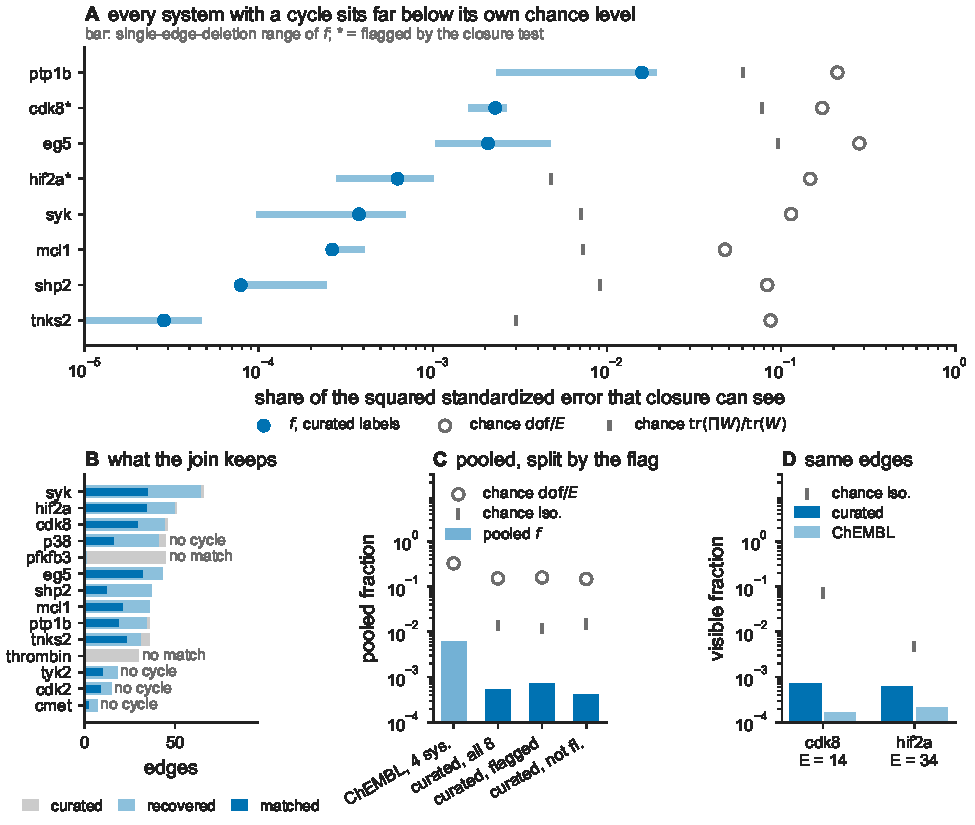
\includegraphics[width=\textwidth]{figGround_curated_grounding.pdf}
\caption{\textbf{The visible fraction of the error against curated experimental labels, over the
benchmark.} (A) Per system with at least one independent cycle in its matched sub-network: the
visible fraction $f$, the range it takes over single-edge deletions, and its two chance levels,
$\mathrm{dof}/E$ and the $\mathrm{tr}(\Pi W)/\mathrm{tr}(W)$ an error isotropic in kcal/mol would
produce under the same projector. An asterisk marks a system the closure test flags. (B) What the
join keeps, per system: curated edges offered, curated edges whose two ligands both recover into
the network, and edges matched into the sub-network the measurement runs on, with the systems that
carry no cycle or no matched edge named. (C) The pooled fraction and its chance levels for all
eight measurable systems and for the flagged and unflagged systems separately, beside the
four-system ChEMBL-grounded figure of Section~\ref{sec:hodge}, which is measured on different
labels and a different edge set and is shown for scale rather than as a comparison. (D) The two
label sources on identical edges, which holds the sub-network fixed: the noisier ChEMBL join gives
the smaller fraction, as a gradient-field label error must.}
\label{fig:Ground}
\end{figure}

\paragraph{The label-noise floor under the visible fraction (Figure~\ref{fig:Noise}).} Experimental
and annotation error is a property of a ligand, so it enters a per-edge error as a difference of
per-ligand terms, $\epsilon_e\to\epsilon_e+b_j-b_i$: a gradient field, which the whitened residual
projector annihilates. Injecting such a field at a per-ligand $\sigma$ of $0.93$ kcal/mol into the
four grounded sub-networks, $200$ seeded draws each, moves the numerator $\|\Pi\tilde\epsilon\|^2$
by at most $1.96\times10^{-11}$ of its own size over all $800$ draws, against a tolerance of
$10^{-10}$ fixed before the measurement was run, and by at most $1.3\times10^{-13}$ measured
against the injected field's own scale; the denominator meanwhile grows by $1.6$ to $2.2\times$ at
the median. Label noise therefore contributes nothing to the numerator of $f$ and all of it to the
denominator, and any correction for it can only move $f$ upward. The $0.6\%$ the main text reports
is a floor on the share of the error attributable to the calculation's own bias, not an estimate of
it.

How much room that leaves is exact arithmetic rather than a fit. If a share $r$ of the measured
per-edge error variance is label noise, the denominator shrinks by $s=1/(1-r)$ and $f$ rises to
$sf$, the numerator being fixed. Pooled, $f$ would first reach its chance level at a shrinkage of
$50.6\times$ in the whitened metric and $14.1\times$ in the isotropic one. That pooled crossing is
not the figure to quote on its own, because per system the room is far from uniform:
\texttt{bace} needs $4.2\times$ whitened and $2.0\times$ isotropic, and under the least
favourable single-edge deletion \texttt{p38} needs $1.46\times$ isotropic and \texttt{bace}
$1.36\times$. Against those, three declared levels of label noise say what a correction could
supply. The first, L1, is the measured literature quantity: mixed public affinity data reproduce
across laboratories at $0.68$ log$_{10}$ units per ligand~\citep{kalliokoski2013mixedic50}, which
at $1.3642$ kcal/mol per log$_{10}$ unit is $0.93$ kcal/mol per ligand and $1.31$ kcal/mol per
edge. L2 and L3 carry half and a quarter of L1's per-edge variance and are stated reductions of it
rather than independent measurements.

The verdict differs by metric, and the metric it fails in is the one the abstract and the main text
quote. In the isotropic metric the bound does not survive a label-noise correction uniformly.
\texttt{bace} isotropic needs $2.00\times$ and L2 supplies $2.55\times$; \texttt{bace} isotropic
under the least favourable single-edge deletion needs $1.36\times$, which both L2 and L3 supply;
\texttt{p38} isotropic under one deletion needs $1.46\times$ and L3, a quarter of the
mixed-laboratory variance, supplies $1.80\times$. A plausible label-noise correction therefore
erases the isotropic reading on those two systems. In the whitened metric the pooled bound needs a
$50.6\times$ shrinkage to be lost and the most any level supplies pooled is $4.13\times$ once each
system is held to its own arithmetic, so there it survives by an order of magnitude; the single
exception is \texttt{bace} under the least favourable single-edge deletion, where the
$2.55\times$ needed and the $2.55\times$ L2 supplies coincide to within one per cent. The bound is therefore
robust to a label-noise correction in the whitened metric the fraction is defined in, and is not
robust in the isotropic metric on \texttt{p38} and \texttt{bace} -- the two systems whose margins
were the weakest before any correction was considered.

The isotropic readings just given stand: L2 and L3 erase them, and nothing here refutes those two
levels. These data do refute L1, the only level with a literature measurement behind it. A
mixed-laboratory per-ligand $\sigma$ of $0.68$ log$_{10}$ implies a label-noise share $r\ge1$ on
\texttt{cdk8}, \texttt{p38} and \texttt{bace}: more label variance than each of those networks'
entire measured error against experiment contains, which is arithmetically impossible, and is
reported as impossible and not clipped. That is direct evidence, from the data and not from an
assumption imported to protect the bound, that $0.68$ log$_{10}$ is an upper bound and not an
estimate for this article's grounding, which takes one ChEMBL target and one assay type per system
and never mixes $\mathrm{IC}_{50}$ with $K_i$.

Two numbers in the same arithmetic land close together without being the same quantity. The
$14.13\times$ that L1 supplies pooled without the per-system cap sits within one per cent of the
$14.08\times$ needed to reach the pooled isotropic chance level. They are different quantities, and
L1 is in any case impossible on three of the four systems taken singly.

None of this measures the label noise in these particular ChEMBL series; it bounds what a
literature-scale label noise could do. A direct measurement would need replicate assay values per
ligand, which the public sources do not carry.

\begin{figure}[t]\centering
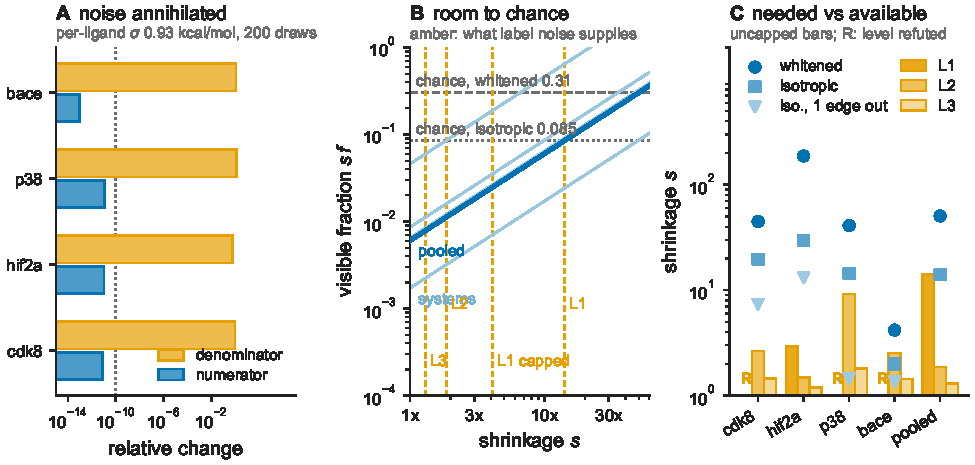
\includegraphics[width=\textwidth]{figNoise_label_noise_floor.pdf}
\caption{\textbf{The label-noise floor under the visible fraction.} (A) A synthetic per-ligand
annotation error of standard deviation $0.93$ kcal/mol is injected into each grounded network as
the gradient field $\epsilon_e\to\epsilon_e+b_j-b_i$, $200$ seeded draws per system: the worst
relative change in the numerator $\|\Pi\tilde\epsilon\|^2$ over all draws, against the median
relative growth of the denominator $\|\tilde\epsilon\|^2$, with the exactness tolerance fixed
before the run marked. (B) The visible fraction under a denominator shrinkage $s$, per system and
pooled, against the pooled whitened and isotropic chance levels; the vertical rules mark the
shrinkage each declared label-noise level supplies. (C) Per system, the shrinkage needed to reach
each chance level -- whitened, isotropic, and isotropic under the least favourable single-edge
deletion -- against the shrinkage each level supplies, uncapped. An R marks a level that asserts
more label variance than that system's whole measured error against experiment contains, and is
therefore refuted by the data rather than truncated.}
\label{fig:Noise}
\end{figure}

The system column carries the benchmark's own name for a target's edge network, which is not a
protein: the $49$ names span $41$ protein labels, \texttt{bace} contributing four and
\texttt{hsp90} four, so a count of flagged systems is not a count of flagged targets. Nor is a name
always one released data set: eight of them combine two or more, which the cross-release
paragraph below takes up. \texttt{ciordia\_retro} is released under the \texttt{asap\_mix} group, and the release's own
statement is the only target assignment used for it.

The component column records the number of connected pieces of a system's edge network. Six of the $48$ systems are disconnected
(\texttt{cdk2}, \texttt{jnk1}, \texttt{mcl1}, \texttt{p38}, \texttt{ptp1b}, \texttt{thrombin}),
each into two pieces, so the components sum to $54$: the benchmark's edge lists join congeneric
series that share a target without joining them to each other. Nothing in the closure statistic is
affected, since $\mathrm{dof}$ is computed as $E$ minus the incidence rank throughout and that
rank already accounts for the extra kernel direction. Elsewhere disconnection does matter. The
offset that Theorem~\ref{thm:hodge}(iv) says the first anchor removes is one offset per component,
so a disconnected system needs one anchor in each piece before any further anchor resolves a
dimension. The grounded networks of Section~\ref{sec:hodge} inherit the same structure, \texttt{cdk8} and
\texttt{bace} being disconnected once restricted to ligands carrying affinities. Their mean
unsigned error against experiment is reported after a single global mean alignment, which is the
conservative convention: aligning each component to its own experimental mean instead, which uses
more experimental information than a prediction has access to, lowers the error by $0.067$ and
$0.014$ kcal/mol respectively and leaves the two connected systems unchanged.

\begin{table}[tp]\centering
\caption{\textbf{What each benchmark system can be audited for.} For the $48$ systems carrying at least one independent cycle: $N$ ligands, $E$ edges, $\nu$ independent cycles, the auditable fraction $\nu/E$ of that system's error space, the number of bridge edges (br), which lie in no cycle and carry no evidence at any magnitude, and the median detectable shift $\tilde\delta^\ast$ in kcal/mol over that system's auditable edges. Rows are ordered by auditable fraction ascending. A dagger marks the eight systems the Benjamini--Hochberg test flags on at least one of the three replicates. Values are replicate-0 and are produced by the same run of the released analysis code that draws Figure~\ref{fig:Hodge}.}
\label{tab:auditability}
\footnotesize
\setlength{\tabcolsep}{3.2pt}
\begin{tabular}{@{}lrrrrrr@{\hspace{10pt}}lrrrrrr@{}}
\toprule
system & $N$ & $E$ & $\nu$ & $\nu/E$ & br & $\tilde\delta^\ast$ & system & $N$ & $E$ & $\nu$ & $\nu/E$ & br & $\tilde\delta^\ast$ \\
\midrule
\texttt{brd4}$^\dagger$ & $8$ & $8$ & $1$ & $0.12$ & $0$ & $0.49$ & \texttt{mcl1} & $54$ & $76$ & $24$ & $0.32$ & $1$ & $0.91$ \\
\texttt{taf12} & $8$ & $8$ & $1$ & $0.12$ & $0$ & $0.48$ & \texttt{hif2a}$^\dagger$ & $41$ & $59$ & $19$ & $0.32$ & $1$ & $0.78$ \\
\texttt{scyt\_dehyd} & $7$ & $7$ & $1$ & $0.14$ & $0$ & $0.43$ & \texttt{shp2} & $26$ & $37$ & $12$ & $0.32$ & $2$ & $1.14$ \\
\texttt{chk1} & $13$ & $15$ & $3$ & $0.20$ & $1$ & $1.29$ & \texttt{syk} & $46$ & $67$ & $22$ & $0.33$ & $5$ & $1.25$ \\
\texttt{t4\_lysozyme} & $12$ & $14$ & $3$ & $0.21$ & $0$ & $0.39$ & \texttt{bace1} & $3$ & $3$ & $1$ & $0.33$ & $0$ & $0.64$ \\
\texttt{hsp90\_kung} & $11$ & $13$ & $3$ & $0.23$ & $0$ & $0.56$ & \texttt{dlk} & $5$ & $6$ & $2$ & $0.33$ & $0$ & $2.09$ \\
\texttt{liga} & $11$ & $13$ & $3$ & $0.23$ & $1$ & $0.95$ & \texttt{factor\_xa} & $3$ & $3$ & $1$ & $0.33$ & $0$ & $2.46$ \\
\texttt{jnk1} & $24$ & $29$ & $7$ & $0.24$ & $3$ & $0.93$ & \texttt{ptp1b} & $26$ & $36$ & $12$ & $0.33$ & $5$ & $1.39$ \\
\texttt{ephx2} & $4$ & $4$ & $1$ & $0.25$ & $0$ & $3.85$ & \texttt{renin}$^\dagger$ & $29$ & $42$ & $14$ & $0.33$ & $0$ & $0.64$ \\
\texttt{hsp90\_single\_ring} & $7$ & $8$ & $2$ & $0.25$ & $0$ & $0.53$ & \texttt{thrombin} & $37$ & $54$ & $19$ & $0.35$ & $0$ & $0.55$ \\
\texttt{hsp90\_woodhead} & $4$ & $4$ & $1$ & $0.25$ & $1$ & $0.37$ & \texttt{keranen\_p2} & $12$ & $17$ & $6$ & $0.35$ & $0$ & $1.27$ \\
\texttt{irak4\_s3} & $4$ & $4$ & $1$ & $0.25$ & $1$ & $1.60$ & \texttt{jak2\_set1} & $10$ & $14$ & $5$ & $0.36$ & $1$ & $0.74$ \\
\texttt{urokinase} & $4$ & $4$ & $1$ & $0.25$ & $0$ & $0.41$ & \texttt{p38}$^\dagger$ & $40$ & $60$ & $22$ & $0.37$ & $5$ & $1.02$ \\
\texttt{tnks2} & $27$ & $35$ & $9$ & $0.26$ & $0$ & $0.47$ & \texttt{hiv1\_protease} & $13$ & $19$ & $7$ & $0.37$ & $0$ & $0.46$ \\
\texttt{faah}$^\dagger$ & $24$ & $31$ & $8$ & $0.26$ & $3$ & $0.88$ & \texttt{cdk2} & $19$ & $27$ & $10$ & $0.37$ & $0$ & $0.92$ \\
\texttt{bace\_ciordia\_prospective} & $9$ & $11$ & $3$ & $0.27$ & $0$ & $0.68$ & \texttt{eg5} & $28$ & $43$ & $16$ & $0.37$ & $3$ & $1.51$ \\
\texttt{bace}$^\dagger$ & $36$ & $49$ & $14$ & $0.29$ & $2$ & $0.57$ & \texttt{btk} & $6$ & $8$ & $3$ & $0.38$ & $0$ & $1.63$ \\
\texttt{bace\_p3\_arg368\_in} & $21$ & $28$ & $8$ & $0.29$ & $8$ & $0.71$ & \texttt{tyk2} & $19$ & $29$ & $11$ & $0.38$ & $1$ & $0.68$ \\
\texttt{hsp90\_2rings} & $6$ & $7$ & $2$ & $0.29$ & $0$ & $0.13$ & \texttt{itk} & $4$ & $5$ & $2$ & $0.40$ & $0$ & $1.24$ \\
\texttt{jak1} & $6$ & $7$ & $2$ & $0.29$ & $1$ & $1.60$ & \texttt{cmet} & $24$ & $39$ & $16$ & $0.41$ & $0$ & $1.12$ \\
\texttt{mup1} & $6$ & $7$ & $2$ & $0.29$ & $0$ & $0.28$ & \texttt{jak2\_set2} & $8$ & $12$ & $5$ & $0.42$ & $0$ & $1.71$ \\
\texttt{hne} & $17$ & $23$ & $7$ & $0.30$ & $0$ & $1.25$ & \texttt{egfr} & $5$ & $7$ & $3$ & $0.43$ & $0$ & $2.90$ \\
\texttt{galectin} & $26$ & $36$ & $11$ & $0.31$ & $0$ & $0.61$ & \texttt{irak4\_s2} & $5$ & $7$ & $3$ & $0.43$ & $0$ & $0.98$ \\
\texttt{ciordia\_retro}$^\dagger$ & $32$ & $45$ & $14$ & $0.31$ & $0$ & $0.68$ & \texttt{cdk8}$^\dagger$ & $35$ & $63$ & $29$ & $0.46$ & $3$ & $0.98$ \\
\bottomrule
\end{tabular}
\end{table}


\paragraph{The cost of a network that can be audited, per system (Table~\ref{tab:design}).} The
design rule of Section~\ref{sec:decomp} is the prospective counterpart of the table above, and
Table~\ref{tab:design} gives it per system. Two kinds of number sit in it and the table keeps them
apart. The augmentation counts $a_b$ and $a_2$, $29$ and $36$ added ligand pairs over the
benchmark, are pure topology: they assume nothing whatever about the edges they add, are certified
minimum against the Eswaran--Tarjan augmentation bound, and were checked independently by brute
force on $39$ of the $40$ (system, target) pairs that need any edge at all, every subset of one
fewer edge failing on each. The further columns, the edges a greedy design adds to bring a system's
median $\delta^\ast$ below $1.0$, $0.75$ and $0.5$ kcal/mol, assume each new edge carries that
system's median reported variance, and are an achievable cost rather than a proven minimum. That
assumption is what the third column of the sensitivity check tests: sweeping the assumed variance
by a factor of two in each direction leaves the verdict and the count stable to within one edge on
$93$ of $96$ system-by-scale comparisons.
Two consequences belong with the rule. Removing bridges buys coverage and not resolution:
on three of the $21$ systems that need any augmentation the median $\delta^\ast$ taken over all
edges is \emph{worse} after augmentation than the median over auditable edges alone that
Table~\ref{tab:auditability} reports, because the bridges that median silently excludes are now
inside it. The second is that $h_e\le1$ pointwise gives $\delta^\ast_e\ge\mathrm{se}_e$, so no
topology can push an edge below its own reported standard error; on a complete graph over $N$ ligands
$h_e=1-2/N$, a second floor for small systems. Measuring every remaining ligand pair still leaves
nine systems above $1.0$ kcal/mol and nineteen above $0.5$, which is the bound of
Theorem~\ref{thm:hodge} appearing in a design question rather than in a diagnostic one.
\begin{table}[tp]\centering
\caption{\textbf{The cost, in added edges, of a network that can be audited.} For the $48$ benchmark systems carrying at least one independent cycle: $E$ edges and the number of bridge edges (br), then two certified-minimum augmentation counts. $a_b$ is the smallest number of new ligand pairs that leaves NO bridge, so that every edge lies on a cycle and carries some evidence; it treats a system's connected components separately, which is all auditability requires, since the closure fit already absorbs one offset per component. $a_2$ additionally joins those components, leaving the whole network 2-edge-connected. Both are pure topology and assume nothing about the new edges. The last three columns are the FURTHER edges a greedy design adds, on top of $a_2$, to bring the median $\delta^\ast$ over that system's own $E$ edges below $1.0$, $0.75$ and $0.5$ kcal/mol, each new edge assumed to carry that system's median reported variance; unlike $a_b$ and $a_2$ these are an achievable cost and not a proven minimum, since the design is greedy. \texttt{--} marks a target no topology can reach, because even measuring every remaining ligand pair leaves the median above it, and $>\!2E$ a target not reached within the explored budget. Across the benchmark $29$ added edges remove all $48$ bridges and $36$ leave every system 2-edge-connected, $2.5\%$ and $3.1\%$ of the $1143$ edges already run. $\delta^\ast$ is the shift at unit noncentrality and not a detection threshold; $80\%$ power at $\alpha=0.05$ needs $2.8$ to $4.7$ times it, so these are targets on a resolution scale. Values are replicate-0 and come from the same run of the released analysis code, \texttt{make figDesign}. A dagger marks the six systems the cycle-closure test flags.}
\label{tab:design}
\footnotesize
\setlength{\tabcolsep}{2.4pt}
\begin{tabular}{@{}lrrrrrrr@{\hspace{6pt}}lrrrrrrr@{}}
\toprule
system & $E$ & br & $a_b$ & $a_2$ & $+1.0$ & $+0.75$ & $+0.5$ & system & $E$ & br & $a_b$ & $a_2$ & $+1.0$ & $+0.75$ & $+0.5$ \\
\midrule
\texttt{p38}$^\dagger$ & $60$ & $5$ & $3$ & $4$ & $1$ & $13$ & -- & \texttt{ciordia\_retro} & $45$ & $0$ & $0$ & $0$ & $0$ & $0$ & $4$ \\
\texttt{bace\_p3\_arg368\_in} & $28$ & $8$ & $3$ & $3$ & $1$ & $1$ & $12$ & \texttt{galectin} & $36$ & $0$ & $0$ & $0$ & $0$ & $0$ & $2$ \\
\texttt{ptp1b} & $36$ & $5$ & $2$ & $3$ & $62$ & -- & -- & \texttt{hiv1\_protease} & $19$ & $0$ & $0$ & $0$ & $0$ & $0$ & $0$ \\
\texttt{cdk2} & $27$ & $0$ & $0$ & $2$ & $0$ & $2$ & $27$ & \texttt{hsp90\_2rings} & $7$ & $0$ & $0$ & $0$ & $0$ & $0$ & $0$ \\
\texttt{cdk8}$^\dagger$ & $63$ & $3$ & $2$ & $2$ & $0$ & $45$ & -- & \texttt{hsp90\_kung} & $13$ & $0$ & $0$ & $0$ & $0$ & $0$ & $1$ \\
\texttt{faah}$^\dagger$ & $31$ & $3$ & $2$ & $2$ & $0$ & $1$ & $8$ & \texttt{hsp90\_single\_ring} & $8$ & $0$ & $0$ & $0$ & $0$ & $0$ & $1$ \\
\texttt{jnk1} & $29$ & $3$ & $2$ & $2$ & $0$ & $2$ & $9$ & \texttt{irak4\_s2} & $7$ & $0$ & $0$ & $0$ & $0$ & -- & -- \\
\texttt{mcl1} & $76$ & $1$ & $1$ & $2$ & $0$ & $1$ & $3$ & \texttt{mup1} & $7$ & $0$ & $0$ & $0$ & $0$ & $0$ & $0$ \\
\texttt{thrombin} & $54$ & $0$ & $0$ & $2$ & $0$ & $0$ & $1$ & \texttt{renin} & $42$ & $0$ & $0$ & $0$ & $0$ & $0$ & $2$ \\
\texttt{syk} & $67$ & $5$ & $2$ & $2$ & $2$ & $5$ & $58$ & \texttt{scyt\_dehyd} & $7$ & $0$ & $0$ & $0$ & $0$ & $0$ & $0$ \\
\texttt{eg5} & $43$ & $3$ & $2$ & $2$ & -- & -- & -- & \texttt{t4\_lysozyme} & $14$ & $0$ & $0$ & $0$ & $0$ & $0$ & $0$ \\
\texttt{bace}$^\dagger$ & $49$ & $2$ & $1$ & $1$ & $0$ & $0$ & $1$ & \texttt{taf12} & $8$ & $0$ & $0$ & $0$ & $0$ & $0$ & $0$ \\
\texttt{hif2a}$^\dagger$ & $59$ & $1$ & $1$ & $1$ & $0$ & $1$ & $12$ & \texttt{tnks2} & $35$ & $0$ & $0$ & $0$ & $0$ & $0$ & $0$ \\
\texttt{hsp90\_woodhead} & $4$ & $1$ & $1$ & $1$ & $0$ & $0$ & $0$ & \texttt{urokinase} & $4$ & $0$ & $0$ & $0$ & $0$ & $0$ & $0$ \\
\texttt{jak2\_set1} & $14$ & $1$ & $1$ & $1$ & $0$ & $0$ & $2$ & \texttt{cmet} & $39$ & $0$ & $0$ & $0$ & $1$ & $16$ & -- \\
\texttt{liga} & $13$ & $1$ & $1$ & $1$ & $0$ & $0$ & $4$ & \texttt{keranen\_p2} & $17$ & $0$ & $0$ & $0$ & $1$ & $3$ & -- \\
\texttt{tyk2} & $29$ & $1$ & $1$ & $1$ & $0$ & $0$ & $2$ & \texttt{btk} & $8$ & $0$ & $0$ & $0$ & $2$ & -- & -- \\
\texttt{chk1} & $15$ & $1$ & $1$ & $1$ & $2$ & $16$ & $24$ & \texttt{hne} & $23$ & $0$ & $0$ & $0$ & $3$ & $>\!2E$ & -- \\
\texttt{shp2} & $37$ & $2$ & $1$ & $1$ & $2$ & $7$ & -- & \texttt{dlk} & $6$ & $0$ & $0$ & $0$ & -- & -- & -- \\
\texttt{irak4\_s3} & $4$ & $1$ & $1$ & $1$ & -- & -- & -- & \texttt{egfr} & $7$ & $0$ & $0$ & $0$ & -- & -- & -- \\
\texttt{jak1} & $7$ & $1$ & $1$ & $1$ & -- & -- & -- & \texttt{ephx2} & $4$ & $0$ & $0$ & $0$ & -- & -- & -- \\
\texttt{bace1} & $3$ & $0$ & $0$ & $0$ & $0$ & $0$ & -- & \texttt{factor\_xa} & $3$ & $0$ & $0$ & $0$ & -- & -- & -- \\
\texttt{bace\_ciordia\_prospective} & $11$ & $0$ & $0$ & $0$ & $0$ & $0$ & $3$ & \texttt{itk} & $5$ & $0$ & $0$ & $0$ & -- & -- & -- \\
\texttt{brd4}$^\dagger$ & $8$ & $0$ & $0$ & $0$ & $0$ & $0$ & $0$ & \texttt{jak2\_set2} & $12$ & $0$ & $0$ & $0$ & -- & -- & -- \\
\bottomrule
\end{tabular}
\end{table}


\paragraph{Between-preparation variance: what the multi-release systems can and cannot supply
(Figure~\ref{fig:Release}).} Three passages of this article need the same missing quantity: the
variance between independent \emph{preparations} of one target, relative to the sampling variance
the reported bar carries. The three are the disagreement with \citet{wade2022estimators} over whether
that bar is conservative, the observation that nothing flags once every bar is widened by half, and
the caveat that the three repeats share one starting structure. The benchmark appears to offer it
in one place. Eight system names union edges from more than one separately released data set, and
where two releases share ligands the union carries cycles that exist in neither release alone,
which close only if the two preparations agree; splitting the closure statistic into its
within-release and across-release blocks would then measure the excess directly. That split, run
over every multi-release system and all three repeats, shows that the public data do not supply the
quantity. Two shared ligands are needed before the union carries an across-release cycle, and only
two of the eight reach that: in the other six (\texttt{cdk2}, \texttt{jnk1},
\texttt{mcl1}, \texttt{p38}, \texttt{ptp1b}, \texttt{thrombin}) the releases share at most one
ligand, the union is disconnected or joined by a tree, and no measurement exists at any magnitude.

Of the two that remain, one is not a join between preparations at all. \texttt{cdk8}'s across-release
block is large, at a reduced $\chi^2$ of $7.77$, $4.79$ and $8.41$ over the three repeats against a
null of exactly $1$, and $5.8$ to $8.2$ times its own within-release block. That excess is the
naming collision of Section~\ref{sec:qc} and not a disagreement between two preparations: its two
releases reuse seven ligand names for chemically different molecules, so every spanning cycle
asserts an equality between distinct ligands. Disambiguating by release removes all six
across-release cycles on every repeat and takes the system's degrees of freedom from $29$ to the
within-release total of $23$, which is the correction this article already applies. The
across-release excess must not be read as a between-preparation estimate, and it is not used as one
anywhere here.

That leaves \texttt{tyk2} as the only genuine cross-release join in the benchmark: two shared
ligands, one across-release cycle. Its across-release block sits at a reduced $\chi^2$ of $0.18$,
$0.70$ and $0.04$ over the three repeats, $p=0.67$ at the first, with a ratio to the within-release
block of $0.2$, $0.6$ and $0.0$. The null it is read against is the right one: synthetic draws on
each system's real topology and real reported bars, with one node potential per shared ligand and
independent noise of the reported size, put \texttt{tyk2}'s block at a mean reduced $\chi^2$ of
$1.069$ over $2000$ draws per repeat, rejecting at $5.7$ to $5.8$ per cent, and \texttt{cdk8}'s at
$1.001$. A second preparation of \texttt{tyk2} therefore adds
nothing detectable beyond sampling, on one cycle, which is far too little to estimate a variance
from. The public data contain no usable estimate of between-preparation variance, and the
disagreement with \citet{wade2022estimators} and the widened-bar observation are scoped by that
absence rather than settled by it. Four further limits apply to any future reading of this split
and none is removable from these data: an across-release block confounds preparation with force
field, protonation, starting structure and mapping, so it bounds the preparation term from above
rather than isolating it; two separately released data sets are not two replicates of one protocol;
the counts are small enough that a single edge moves them, which the leave-one-edge-out ranges
emitted with the figure quantify; and the split is not independent of what this article already reports,
since the one system carrying most of the arithmetic is one the closure test already flags for the
reason given above.

\begin{figure}[t]\centering
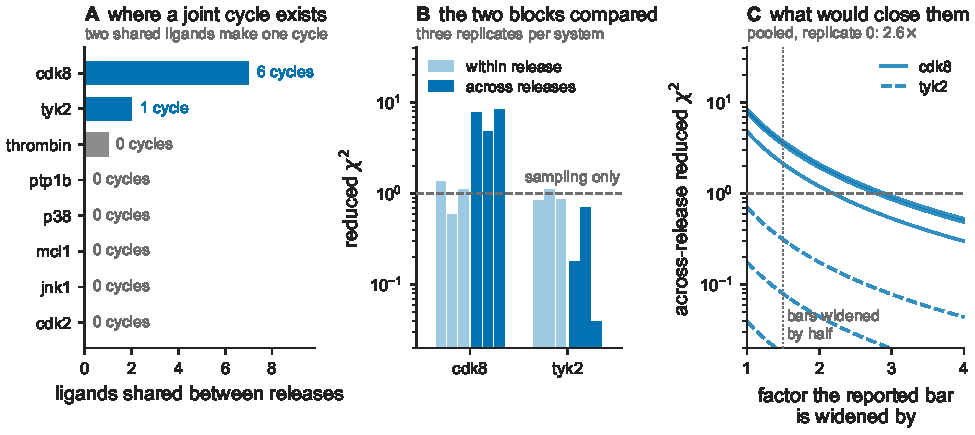
\includegraphics[width=\textwidth]{figRelease_cross_release_variance.pdf}
\caption{\textbf{What the multi-release systems can measure about between-preparation variance.}
(A) For each system name that unions more than one separately released data set, the largest number
of ligands any two of its releases share, annotated with the number of across-release cycles that
creates. Two shared ligands are needed for one cycle. (B) Within-release and across-release reduced
$\chi^2$ for the two systems that carry an across-release cycle, three protocol repeats each,
against the value sampling alone would give. (C) The across-release reduced $\chi^2$ of the same
two systems as every reported standard error is widened by a common factor, with the half-again
widening of the main text's stress test marked; scaling every bar by $\lambda$ divides the
statistic by $\lambda^2$ exactly and leaves the fit unchanged. \texttt{cdk8}'s block measures a
reuse of seven ligand names for different molecules between its two releases, not a disagreement
between two preparations, and is not a between-preparation reading.}
\label{fig:Release}
\end{figure}

\begin{figure}[t]\centering
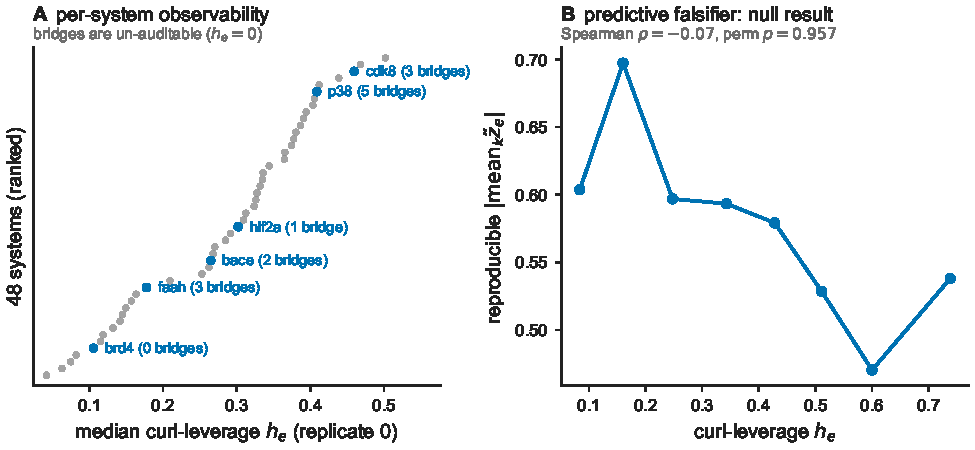
\includegraphics[width=\textwidth]{figLev_observability.pdf}
\caption{\textbf{Per-system curl-leverage, and curl-leverage versus reproducible residual
magnitude.} (A) Median curl-leverage $h_e$ per system, ranked, across the $48$ systems with
at least one independent cycle; the six cycle-closure-flagged systems are labeled with their
number of bridge ($h_e=0$) edges. (B) Curl-leverage $h_e$, binned into $8$ quantiles, versus
the mean studentized cross-replicate reproducible residual magnitude in each bin, with the
Spearman correlation and permutation $p$-value.}
\label{fig:Lev}
\end{figure}

\paragraph{Close-the-loop accuracy comparison (Figure~\ref{fig:Lcausal}).} On the four flagged systems
groundable against public ChEMBL affinity, guided removal of the QC-flagged high-$|z|$ edges ties a
size-matched random removal on MUE-vs-experiment (combined Stouffer $p=0.48$). Removing the
highest-$|z|$ edges lowers the closure statistic (Figure~\ref{fig:Lval}A), but that is
arithmetic and not evidence, because the statistic is the sum of exactly the per-edge quantities
being removed in descending order (Section~\ref{sec:qc}). The comparison adds that the same removal yields no improvement against
experiment. The reach demonstrated for the closure test therefore stops at internal
edge-level consistency and does not extend to force-field-limited absolute accuracy, the same
scope boundary as the clean \texttt{eg5} system. Throughout, $\Delta$MUE is oriented as
$\mathrm{MUE}(\text{full})-\mathrm{MUE}(\text{after})$, the same orientation as
Figure~\ref{fig:Hodge}C.

\begin{figure}[t]\centering
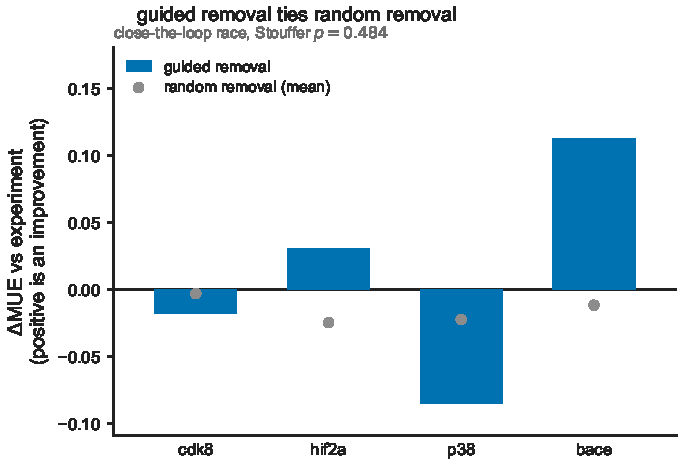
\includegraphics[width=0.7\textwidth]{figLcausal_guided_vs_random.pdf}
\caption{\textbf{Change in mean unsigned error against experimental affinity after guided
versus random QC-edge removal.} Bars: change in mean unsigned error against experiment
($\Delta$MUE) after guided removal of the QC-flagged high-$|z|$ edges, per system. Points:
mean $\Delta$MUE after a size-matched random removal, per system. Throughout, $\Delta$MUE is
$\mathrm{MUE}(\text{full})-\mathrm{MUE}(\text{after})$, so a positive value is an improvement. Systems: \texttt{cdk8},
\texttt{hif2a}, \texttt{p38}, \texttt{bace}.}
\label{fig:Lcausal}
\end{figure}

\paragraph{Fixed-cutoff head-to-head and $\chi^2$ reconciliation (Figure~\ref{fig:Cut}).} Two
pre-registered checks were run on the same $1143$ edges of the $48$ cyclic systems. The first
is the head-to-head: the calibrated test, scored by area under the
receiver-operating-characteristic curve (AUC) against the reproducible-systematic magnitude
defined in Computational details,
scores $0.865$. Against a fixed $1.0$ kcal/mol hysteresis cutoff's $0.575$ the paired bootstrap
difference is $+0.290$ $[+0.094,+0.490]$; against a fixed-$\mathrm{se}$ $\chi^2$ test's $0.725$ it
is $+0.140$ $[-0.008,+0.316]$, straddling zero. The pre-registered criterion required the
calibrated test to exceed both, so the verdict is a tie. The ordering within that tie is not a discrimination gain over the fixed cutoff in standard use: the scored label standardizes each residual by the same per-edge reported variance the calibrated rule weights by, so the AUC ordering is monotone in a rule's proximity to that variance and the comparison ranks nothing. The second check tested whether
correlation among residuals of edges sharing a ligand endpoint explains the apparent gap between
the inverted-median factor, $1.71\times$ obtained as $1/\sqrt{0.34}$ from the median reduced
$\chi^2$, and the replicate ratio of $1.41\times$ measured against seed and velocity repeats. It
does not: the excess correlation is $-0.0079$ $[-0.0314,+0.0164]$, and the Benjamini--Hochberg flag
set is unchanged.

The two inverted-median factors quoted in this article are the same functional on two populations
and do not conflict. The pre-registered constant $1.71\times$ is $1/\sqrt{0.34}$ from the median
reduced $\chi^2$ over all $48$ cyclic systems, the population of Figure~\ref{fig:L}; the
$1.67\times$ annotated inside panel B is $1/\sqrt{0.361}$ over the $46$ systems this second check
admits, since estimating the shared-node null needs at least one disjoint edge pair per system and
\texttt{bace1} and \texttt{factor\_xa} are three-edge triangles that have none. Dropping those two
raises the median.

Neither the pre-registered constant nor the factor annotated in panel B is a conservatism estimate,
because the premise of the second check is unsound: by Theorem~\ref{thm:cons} the closure statistic
identifies the closure-weighted mean of $c_e^{-2}$ and not a median, so
$1/\sqrt{\mathrm{median}}$ does not estimate the same functional as the replicate ratio. There is
accordingly no physical gap for shared-node correlation to explain. The pre-registered constants
are retained as the pre-registered record, and the verdict above is reported as run and not
revised. On replicate $0$ the calibrated test flags $6$ of $48$
systems, the fixed-$\mathrm{se}$ $\chi^2$ test $11$, and the fixed cutoff $26$, and the three flag
sets are strictly nested (calibrated $\subset$ fixed-$\mathrm{se}$ $\subset$ fixed cutoff), so on
that replicate the calibrated test catches no system the fixed cutoff misses and instead removes
$20$ of its flags. The strict chain is a property of that replicate and not of the benchmark. On
replicate $1$ the counts are $6$, $13$ and $24$ and two links fail: \texttt{ciordia\_retro} is
flagged by the calibrated test and not by the fixed-$\mathrm{se}$ test, and \texttt{mup1} by the
fixed-$\mathrm{se}$ test and not by the cutoff. On replicate $2$ the counts are $3$, $11$ and $24$
and the chain holds. The calibrated set lies inside the cutoff's on all three, which is the only
containment any claim here rests on. Under the release's own blocks rather than the by-target
grouping, the same replicate-$0$ test over $56$ testable blocks gives $6$, $10$ and $29$, the chain
nests, and the calibrated test removes $23$ of the cutoff's flags. Whether that removal is an improvement is what the head-to-head above cannot determine, for the
reason given there. The $1.0$ kcal/mol cutoff was pre-registered at the
field-standard value before this comparison was run, and no sweep over alternative thresholds
was performed, so the comparison above is specific to that one fixed rule.

\begin{figure}[t]\centering
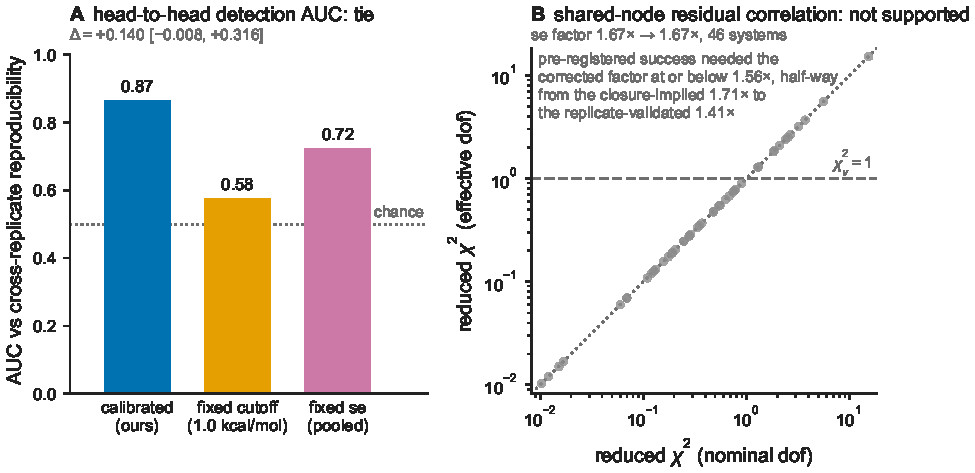
\includegraphics[width=\textwidth]{figCut_cutoff_benchmark.pdf}
\caption{\textbf{Detection AUC of three flagging rules, and nominal versus
correlation-corrected reduced $\chi^2$.} (A) Area under the ROC curve (AUC) scored against the
per-system reproducible-systematic magnitude defined in Computational details, for the calibrated
per-edge null, a fixed $1.0$
kcal/mol hysteresis cutoff, and a fixed-standard-error $\chi^2$ test, with the chance level
($\mathrm{AUC}=0.5$) marked. (B) Per-system reduced $\chi^2$ at the nominal degrees of
freedom versus at the shared-node-correlation-corrected effective degrees of freedom, with the
$y{=}x$ line, the $\chi^2_\nu=1$ reference, and the annotated inverted-median factor of
$1.67\times$, the pre-registered functional evaluated over this panel's $46$ systems.}
\label{fig:Cut}
\end{figure}

\begin{figure}[t]\centering
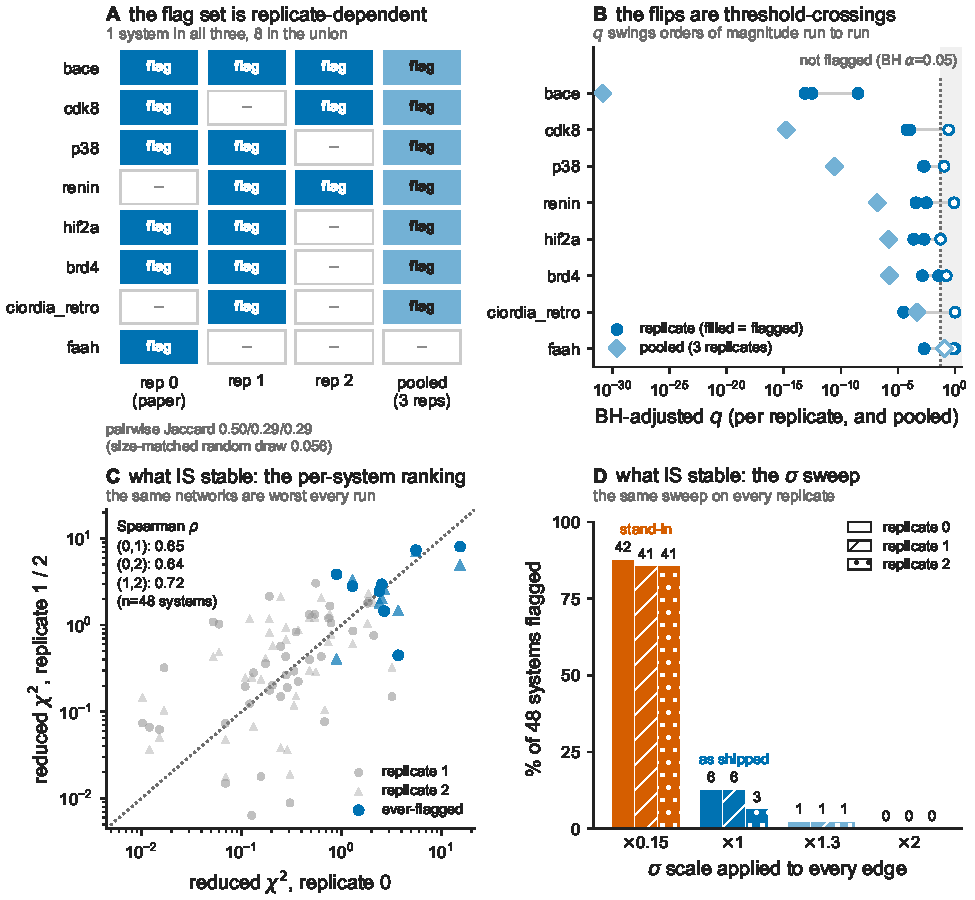
\includegraphics[width=\textwidth]{figStab_replicate_stability.pdf}
\caption{\textbf{Replicate stability of the flag set.} The Benjamini--Hochberg test at
$\alpha=0.05$ recomputed independently on each of the benchmark's three protocol repeats.
Per-system adjusted $p$-values, which systems are flagged on which replicate, the pairwise
Jaccard overlap of the three flag sets against a random-draw reference, the flag set obtained
from the three replicates pooled, and the selectivity of the test across a swept uniform
$\sigma$ scale on each replicate.}
\label{fig:Stab}
\end{figure}

\paragraph{The flag sets under arbitrary dependence (Figure~\ref{fig:Stab}).} The correction
reported throughout is Benjamini--Hochberg, whose guarantee needs a dependence assumption between
systems. Benjamini--Yekutieli~\citep{benjamini2001by} needs none, at the cost of running the same
step-up rule at $\alpha/H_m$ with $H_{48}=4.4588$, that is at $0.0112$ rather than $0.05$. It
returns $\{$\texttt{bace}, \texttt{brd4}, \texttt{cdk8}, \texttt{faah}, \texttt{hif2a},
\texttt{p38}$\}$ on replicate $0$, identical to the published set; $\{$\texttt{bace},
\texttt{cdk8}, \texttt{renin}$\}$ on replicate $2$, again identical; and on replicate $1$
$\{$\texttt{bace}, \texttt{ciordia\_retro}, \texttt{hif2a}, \texttt{p38}, \texttt{renin}$\}$,
which drops \texttt{brd4} from the Benjamini--Hochberg set of six. The published set therefore does
not depend on the dependence assumption, and the variation of the flag set across replicates is
unchanged by removing it. \texttt{make figStab} emits the three sets.

\paragraph{Per-system test statistics behind the flag sets (Tables~\ref{tab:stab}
and~\ref{tab:stab2}).} The flag sets summarized in Figure~\ref{fig:Stab} and in
Section~\ref{sec:stability} are thresholded Benjamini--Hochberg adjusted $p$-values, so the
underlying continuous quantities are reported in full rather than only their dichotomization.
For each system, a generalized-least-squares cycle-closure fit under the calibrated per-edge
null gives a $\chi^2$ on $\nu$ degrees of freedom, $\nu$ being the number of independent cycles
in that system's edge network; the reduced value $\chi^2_\nu=\chi^2/\nu$ and the raw upper-tail
probability follow, and those raw $p$-values are corrected for testing $48$ systems by the
Benjamini--Hochberg procedure at a false-discovery rate of $0.05$, giving the adjusted
$q$-values tabulated below. The $q\le0.05$ rule reproduces the released implementation exactly, and that correspondence is asserted on every set the analysis emits.
Each of the benchmark's three protocol replicates is analysed independently: the fit is rerun
from scratch on that replicate's edges and the correction is applied within that replicate
alone, so the three $q$ columns are not a joint error rate across replicates. All values in both
parts of the table are produced by the same run of the released analysis code that draws
Figure~\ref{fig:Stab}.

\begin{table}[tp]\centering
\caption{\textbf{Per-system cycle-closure statistics and Benjamini--Hochberg adjusted
$q$-values, per replicate (part $1$ of $2$).} Reduced $\chi^2$ and adjusted $q$-value from the
calibrated cycle-closure test at a false-discovery rate of $0.05$, computed independently on each
of the three protocol replicates, for the $48$ systems with at least one independent cycle;
$\nu$ is the number of independent cycles. Bold marks $q\le0.05$; the final column lists the
replicates on which the system is flagged, and a dash where it never is. Edge and cycle counts are
the replicate-0 values. Rows are ordered by replicate-0 $q$ ascending. The remaining $24$ systems
continue in Table~\ref{tab:stab2}.}
\label{tab:stab}
\footnotesize
\setlength{\tabcolsep}{3.4pt}
\begin{tabular}{@{}lrrrrrrrrc@{}}
\toprule
& & & \multicolumn{2}{c}{replicate 0} & \multicolumn{2}{c}{replicate 1} &
\multicolumn{2}{c}{replicate 2} & \\
\cmidrule(lr){4-5}\cmidrule(lr){6-7}\cmidrule(lr){8-9}
system & edges & $\nu$ & $\chi^2_\nu$ & $q$ & $\chi^2_\nu$ & $q$ & $\chi^2_\nu$ & $q$ &
flagged \\
\midrule
\texttt{bace} & $49$ & $14$ & $\mathbf{5.57}$ & $\mathbf{3.2{\times}10^{-9}}$ & $\mathbf{7.33}$ & $\mathbf{7.0{\times}10^{-14}}$ & $\mathbf{7.10}$ & $\mathbf{2.9{\times}10^{-13}}$ & 0, 1, 2 \\
\texttt{cdk8} & $63$ & $29$ & $\mathbf{2.68}$ & $\mathbf{6.1{\times}10^{-5}}$ & $1.45$ & $2.8{\times}10^{-1}$ & $\mathbf{2.62}$ & $\mathbf{1.1{\times}10^{-4}}$ & 0, 2 \\
\texttt{brd4} & $8$ & $1$ & $\mathbf{15.40}$ & $\mathbf{1.4{\times}10^{-3}}$ & $\mathbf{8.05}$ & $\mathbf{3.6{\times}10^{-2}}$ & $4.94$ & $1.7{\times}10^{-1}$ & 0, 1 \\
\texttt{faah} & $31$ & $8$ & $\mathbf{3.71}$ & $\mathbf{2.0{\times}10^{-3}}$ & $0.45$ & $1.0{\times}10^{0}$ & $1.47$ & $7.1{\times}10^{-1}$ & 0 \\
\texttt{hif2a} & $59$ & $19$ & $\mathbf{2.53}$ & $\mathbf{2.0{\times}10^{-3}}$ & $\mathbf{2.96}$ & $\mathbf{2.4{\times}10^{-4}}$ & $2.05$ & $5.4{\times}10^{-2}$ & 0, 1 \\
\texttt{p38} & $60$ & $22$ & $\mathbf{2.40}$ & $\mathbf{2.0{\times}10^{-3}}$ & $\mathbf{2.48}$ & $\mathbf{1.7{\times}10^{-3}}$ & $1.81$ & $1.1{\times}10^{-1}$ & 0, 1 \\
\texttt{mcl1} & $76$ & $24$ & $1.82$ & $5.5{\times}10^{-2}$ & $1.79$ & $6.8{\times}10^{-2}$ & $1.04$ & $1.0{\times}10^{0}$ & -- \\
\texttt{bace\_p3\_arg368\_in} & $28$ & $8$ & $1.88$ & $3.5{\times}10^{-1}$ & $1.88$ & $2.8{\times}10^{-1}$ & $2.32$ & $1.4{\times}10^{-1}$ & -- \\
\texttt{taf12} & $8$ & $1$ & $3.21$ & $3.9{\times}10^{-1}$ & $0.15$ & $1.0{\times}10^{0}$ & $0.33$ & $1.0{\times}10^{0}$ & -- \\
\texttt{liga} & $13$ & $3$ & $2.10$ & $4.7{\times}10^{-1}$ & $0.76$ & $1.0{\times}10^{0}$ & $1.80$ & $6.9{\times}10^{-1}$ & -- \\
\texttt{thrombin} & $54$ & $19$ & $1.30$ & $7.4{\times}10^{-1}$ & $0.86$ & $1.0{\times}10^{0}$ & $0.61$ & $1.0{\times}10^{0}$ & -- \\
\texttt{renin} & $42$ & $14$ & $1.29$ & $8.1{\times}10^{-1}$ & $\mathbf{2.81}$ & $\mathbf{3.1{\times}10^{-3}}$ & $\mathbf{3.32}$ & $\mathbf{3.8{\times}10^{-4}}$ & 1, 2 \\
\texttt{ciordia\_retro} & $45$ & $14$ & $0.89$ & $1.0{\times}10^{0}$ & $\mathbf{3.86}$ & $\mathbf{3.1{\times}10^{-5}}$ & $0.40$ & $1.0{\times}10^{0}$ & 1 \\
\texttt{tyk2} & $29$ & $11$ & $0.79$ & $1.0{\times}10^{0}$ & $1.06$ & $1.0{\times}10^{0}$ & $0.78$ & $1.0{\times}10^{0}$ & -- \\
\texttt{ephx2} & $4$ & $1$ & $0.77$ & $1.0{\times}10^{0}$ & $1.67$ & $7.7{\times}10^{-1}$ & $1.33$ & $9.3{\times}10^{-1}$ & -- \\
\texttt{shp2} & $37$ & $12$ & $0.74$ & $1.0{\times}10^{0}$ & $1.21$ & $8.7{\times}10^{-1}$ & $0.64$ & $1.0{\times}10^{0}$ & -- \\
\texttt{itk} & $5$ & $2$ & $0.68$ & $1.0{\times}10^{0}$ & $0.08$ & $1.0{\times}10^{0}$ & $0.10$ & $1.0{\times}10^{0}$ & -- \\
\texttt{tnks2} & $35$ & $9$ & $0.63$ & $1.0{\times}10^{0}$ & $0.43$ & $1.0{\times}10^{0}$ & $2.07$ & $1.7{\times}10^{-1}$ & -- \\
\texttt{mup1} & $7$ & $2$ & $0.55$ & $1.0{\times}10^{0}$ & $3.05$ & $2.8{\times}10^{-1}$ & $0.29$ & $1.0{\times}10^{0}$ & -- \\
\texttt{scyt\_dehyd} & $7$ & $1$ & $0.54$ & $1.0{\times}10^{0}$ & $1.34$ & $8.5{\times}10^{-1}$ & $1.23$ & $9.3{\times}10^{-1}$ & -- \\
\texttt{cdk2} & $27$ & $10$ & $0.48$ & $1.0{\times}10^{0}$ & $1.33$ & $7.7{\times}10^{-1}$ & $1.22$ & $9.3{\times}10^{-1}$ & -- \\
\texttt{eg5} & $43$ & $16$ & $0.48$ & $1.0{\times}10^{0}$ & $0.40$ & $1.0{\times}10^{0}$ & $0.30$ & $1.0{\times}10^{0}$ & -- \\
\texttt{galectin} & $36$ & $11$ & $0.37$ & $1.0{\times}10^{0}$ & $0.22$ & $1.0{\times}10^{0}$ & $0.88$ & $1.0{\times}10^{0}$ & -- \\
\texttt{jak2\_set1} & $14$ & $5$ & $0.35$ & $1.0{\times}10^{0}$ & $0.83$ & $1.0{\times}10^{0}$ & $0.15$ & $1.0{\times}10^{0}$ & -- \\
\bottomrule
\end{tabular}
\end{table}

\begin{table}[tp]\centering
\caption{\textbf{Per-system cycle-closure statistics and Benjamini--Hochberg adjusted
$q$-values, per replicate (part $2$ of $2$).} Table~\ref{tab:stab} continued: the remaining $24$
of the $48$ systems, in the same order and with the same conventions. No system in this part is
flagged on any replicate.}
\label{tab:stab2}
\footnotesize
\setlength{\tabcolsep}{3.4pt}
\begin{tabular}{@{}lrrrrrrrrc@{}}
\toprule
& & & \multicolumn{2}{c}{replicate 0} & \multicolumn{2}{c}{replicate 1} &
\multicolumn{2}{c}{replicate 2} & \\
\cmidrule(lr){4-5}\cmidrule(lr){6-7}\cmidrule(lr){8-9}
system & edges & $\nu$ & $\chi^2_\nu$ & $q$ & $\chi^2_\nu$ & $q$ & $\chi^2_\nu$ & $q$ &
flagged \\
\midrule
\texttt{hsp90\_2rings} & $7$ & $2$ & $0.34$ & $1.0{\times}10^{0}$ & $0.29$ & $1.0{\times}10^{0}$ & $0.12$ & $1.0{\times}10^{0}$ & -- \\
\texttt{factor\_xa} & $3$ & $1$ & $0.31$ & $1.0{\times}10^{0}$ & $0.01$ & $1.0{\times}10^{0}$ & $0.02$ & $1.0{\times}10^{0}$ & -- \\
\texttt{keranen\_p2} & $17$ & $6$ & $0.29$ & $1.0{\times}10^{0}$ & $0.19$ & $1.0{\times}10^{0}$ & $0.04$ & $1.0{\times}10^{0}$ & -- \\
\texttt{chk1} & $15$ & $3$ & $0.28$ & $1.0{\times}10^{0}$ & $0.27$ & $1.0{\times}10^{0}$ & $0.69$ & $1.0{\times}10^{0}$ & -- \\
\texttt{hiv1\_protease} & $19$ & $7$ & $0.28$ & $1.0{\times}10^{0}$ & $0.43$ & $1.0{\times}10^{0}$ & $0.94$ & $1.0{\times}10^{0}$ & -- \\
\texttt{irak4\_s2} & $7$ & $3$ & $0.25$ & $1.0{\times}10^{0}$ & $0.15$ & $1.0{\times}10^{0}$ & $0.04$ & $1.0{\times}10^{0}$ & -- \\
\texttt{t4\_lysozyme} & $14$ & $3$ & $0.25$ & $1.0{\times}10^{0}$ & $0.57$ & $1.0{\times}10^{0}$ & $2.14$ & $5.0{\times}10^{-1}$ & -- \\
\texttt{ptp1b} & $36$ & $12$ & $0.21$ & $1.0{\times}10^{0}$ & $0.20$ & $1.0{\times}10^{0}$ & $0.58$ & $1.0{\times}10^{0}$ & -- \\
\texttt{btk} & $8$ & $3$ & $0.19$ & $1.0{\times}10^{0}$ & $2.15$ & $4.0{\times}10^{-1}$ & $1.19$ & $9.3{\times}10^{-1}$ & -- \\
\texttt{hsp90\_kung} & $13$ & $3$ & $0.19$ & $1.0{\times}10^{0}$ & $0.18$ & $1.0{\times}10^{0}$ & $0.83$ & $1.0{\times}10^{0}$ & -- \\
\texttt{cmet} & $39$ & $16$ & $0.17$ & $1.0{\times}10^{0}$ & $0.36$ & $1.0{\times}10^{0}$ & $0.42$ & $1.0{\times}10^{0}$ & -- \\
\texttt{hsp90\_single\_ring} & $8$ & $2$ & $0.16$ & $1.0{\times}10^{0}$ & $0.02$ & $1.0{\times}10^{0}$ & $0.24$ & $1.0{\times}10^{0}$ & -- \\
\texttt{hne} & $23$ & $7$ & $0.13$ & $1.0{\times}10^{0}$ & $0.28$ & $1.0{\times}10^{0}$ & $0.07$ & $1.0{\times}10^{0}$ & -- \\
\texttt{urokinase} & $4$ & $1$ & $0.13$ & $1.0{\times}10^{0}$ & $0.01$ & $1.0{\times}10^{0}$ & $0.25$ & $1.0{\times}10^{0}$ & -- \\
\texttt{jnk1} & $29$ & $7$ & $0.12$ & $1.0{\times}10^{0}$ & $0.12$ & $1.0{\times}10^{0}$ & $1.19$ & $9.3{\times}10^{-1}$ & -- \\
\texttt{syk} & $67$ & $22$ & $0.11$ & $1.0{\times}10^{0}$ & $0.20$ & $1.0{\times}10^{0}$ & $0.25$ & $1.0{\times}10^{0}$ & -- \\
\texttt{egfr} & $7$ & $3$ & $0.07$ & $1.0{\times}10^{0}$ & $0.01$ & $1.0{\times}10^{0}$ & $0.02$ & $1.0{\times}10^{0}$ & -- \\
\texttt{irak4\_s3} & $4$ & $1$ & $0.07$ & $1.0{\times}10^{0}$ & $0.07$ & $1.0{\times}10^{0}$ & $0.05$ & $1.0{\times}10^{0}$ & -- \\
\texttt{jak2\_set2} & $12$ & $5$ & $0.06$ & $1.0{\times}10^{0}$ & $1.02$ & $1.0{\times}10^{0}$ & $0.49$ & $1.0{\times}10^{0}$ & -- \\
\texttt{bace1} & $3$ & $1$ & $0.05$ & $1.0{\times}10^{0}$ & $1.09$ & $8.9{\times}10^{-1}$ & $0.43$ & $1.0{\times}10^{0}$ & -- \\
\texttt{dlk} & $6$ & $2$ & $0.02$ & $1.0{\times}10^{0}$ & $0.06$ & $1.0{\times}10^{0}$ & $0.05$ & $1.0{\times}10^{0}$ & -- \\
\texttt{jak1} & $7$ & $2$ & $0.02$ & $1.0{\times}10^{0}$ & $0.32$ & $1.0{\times}10^{0}$ & $0.10$ & $1.0{\times}10^{0}$ & -- \\
\texttt{bace\_ciordia\_prospective} & $11$ & $3$ & $0.01$ & $1.0{\times}10^{0}$ & $0.07$ & $1.0{\times}10^{0}$ & $0.04$ & $1.0{\times}10^{0}$ & -- \\
\texttt{hsp90\_woodhead} & $4$ & $1$ & $0.01$ & $1.0{\times}10^{0}$ & $0.07$ & $1.0{\times}10^{0}$ & $0.15$ & $1.0{\times}10^{0}$ & -- \\
\bottomrule
\end{tabular}
\end{table}

\paragraph{Out-of-sample behaviour of the calibrated null (Figure~\ref{fig:OOS}).} Each candidate
held-out statistic is calibrated against a no-error null before use, and the realized level of
every candidate is reported. Two of the candidates fire far above nominal and are not used; the
remaining two hold their nominal level and are the ones carried into the selection comparisons.

\begin{figure}[t]\centering
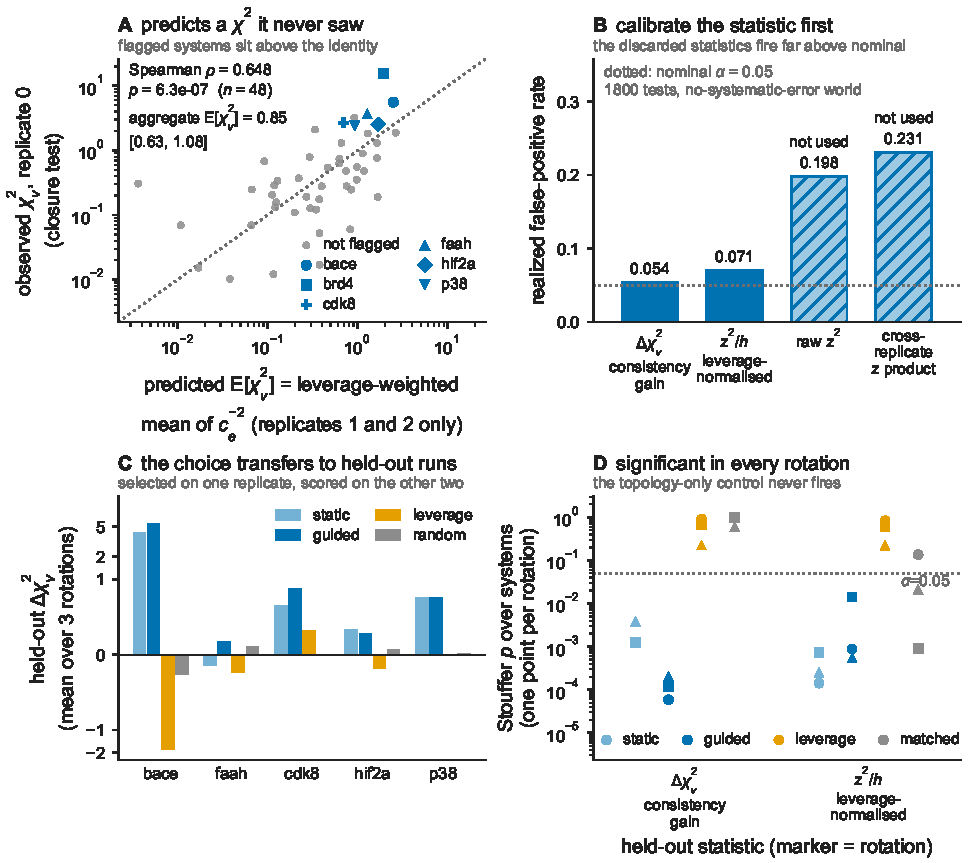
\includegraphics[width=\textwidth]{figOOS_out_of_sample.pdf}
\caption{\textbf{Out-of-sample behaviour of the calibrated null.} (A) Per-system closure
$\chi^2_\nu$ predicted from the per-edge miscalibration measured on the two replicates not being
predicted, against the observed value, with the identity line and the flagged systems marked.
(B) Realized false-positive rate of each candidate held-out statistic under a simulation with no
systematic error anywhere, against the nominal level, with the two statistics that fire far above
nominal marked. (C) Held-out change in reduced $\chi^2$ on the two
replicates not used for selection, after removing the edges selected on the third, averaged over
the three rotations and shown per testable flagged system, for a static and a guided selection
rule, a topology-only rule built from curl-leverage, and equal-size random removal. (D)
Stouffer-combined $p$-value over systems, one point per rotation, for each of the two statistics
that held their nominal level, under the same selection rules together with an $|z|$-rank-matched
control drawn from unflagged systems, with the $\alpha=0.05$ line marked.}
\label{fig:OOS}
\end{figure}

\paragraph{Two-sided self-calibration of the per-edge error bar (Figure~\ref{fig:Self}).} Seven arms
are compared: the nominal test, which uses the reported standard errors unchanged; the two-sided
correction at the pre-specified per-edge granularity, which corrects each edge by its own ratio; a
coarser variant correcting each system by its aggregate ratio; a variant clipping the ratio to
$[1/3,3]$; a variant dividing the replicate standard deviation by the constant $c_4(3)=0.886$, the
expectation of the sample standard deviation at three draws, which widens the bars; a variant
measuring the ratio on the two replicates the test does not read; and, at the same per-edge
granularity, the one-sided correction that inflates only where the measurement says the bar is too
tight, which is the direction of Table~\ref{tab:P8} applied per edge rather than per system. The
constant $c_4(3)$ is unrelated to the per-edge calibration ratio $c_e$.
Table~\ref{tab:selfgrid} tabulates the four granularity-by-direction combinations.

\begin{figure}[t]\centering
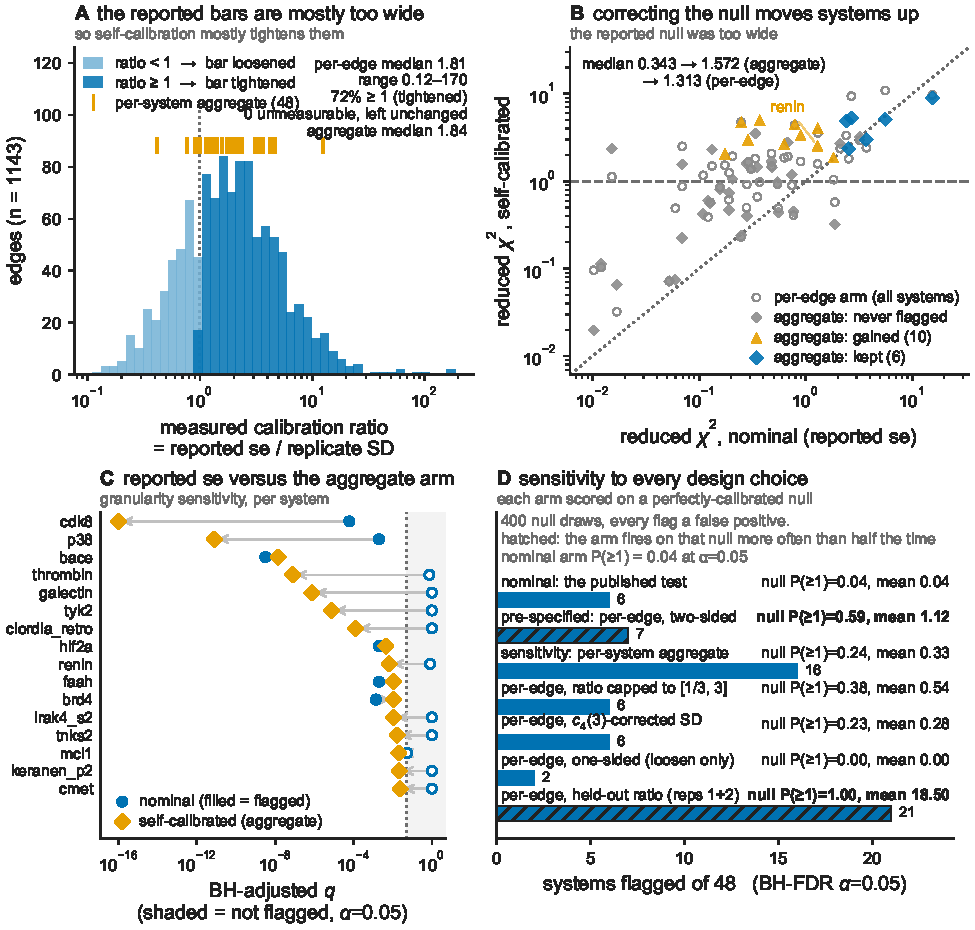
\includegraphics[width=\textwidth]{figSelf_two_sided_selfcalibration.pdf}
\caption{\textbf{Two-sided self-calibration of the per-edge error bar.} Per-system reduced
$\chi^2$ before and after replacing each system's reported standard error by its own
replicate-measured calibration, which systems are gained and which are lost, and the realized
probability of at least one false flag for each arm under a pure-null simulation, for the seven
arms described in the text.}
\label{fig:Self}
\end{figure}

\paragraph{Simulation protocols.} The two protocols the main text names are specified here.

\paragraph{The pure-null simulation behind the realized levels.} Every realized level quoted for a
self-calibrated arm, in Section~\ref{sec:qc}, in Section~\ref{sec:limitations} and in the last
column of Supplementary Table~\ref{tab:selfgrid}, is measured on a synthetic benchmark that carries
no systematic error, so that every flag it produces is a false positive by construction. The
topologies are the real ones: the same $48$ systems the closure test admits, each with its own
ligand-pair edge list and its own admission by the same rule ($\geq3$ edges, $\geq1$ independent
cycle), which depends on topology alone. The variances are the real ones: each edge keeps the
per-edge reported standard error it carries, and that value is then declared to be the
edge's true sampling standard deviation, which makes the reported bars perfectly calibrated by
construction. The draw law is the null: every node potential is exact, so each edge's true
$\ddG$ is exactly the difference of its endpoints' potentials, and an observation is that value
plus an independent Gaussian of the edge's own standard deviation. There is no systematic
component anywhere and no correlation between edges. The replicate structure mirrors the
benchmark's: three independent draws per edge, of which the first plays the role of replicate $0$
and is the one the closure statistic is computed on, while all three are read by the arm's own
calibration formula exactly as that arm reads the real replicates (the held-out arm reads only the
second and third). Each arm's correction, tail probability and Benjamini--Hochberg step-up at
$\alpha=0.05$ are then the identical code paths used on the real data. The simulation is run for
$400$ draws, so a realized probability is measured to a Monte-Carlo standard error of at most
$\sqrt{0.25/400}=0.025$, and the generator is seeded once for the whole sweep, which makes the
reported levels reproducible.

\paragraph{The reproducible-systematic magnitude used as ground truth.} Detection comparisons
need a label that does not come from the detector being scored, and the only one these data
supply is reproduction across the three protocol repeats. It is defined as follows. Each
replicate's network is fitted separately by the same generalized least squares, giving for
replicate $k$ and edge $e$ a standardized residual $z_e^{(k)}=r_e^{(k)}/\sqrt{V_e^{\mathrm{rep}}}$.
The three signed residuals of an edge are averaged, $\bar z_e=\frac13\sum_k z_e^{(k)}$, so
that a residual reproducing in sign and magnitude survives the average while sampling noise
cancels toward zero, and the edge's score is $|\bar z_e|$. A system's score is the median of
$|\bar z_e|$ over its edges. This is the quantity the detectors of the head-to-head comparison
are ranked against, by Mann--Whitney AUC of the binary flag against the per-system score. It uses
only replicate residuals and no detector output, but it is not independent of the rules being
scored, and the dependence is the reason no ordering is read out of that comparison
(Section~\ref{sec:qc}): $z_e^{(k)}$ divides by $V_e^{\mathrm{rep}}$, the same per-edge reported
variance the calibrated rule uses as its weight, so the label rewards a rule for standing close to
that variance. ``Edges whose sign and magnitude
reproduce across independent replicates'', wherever that phrase appears above, means edges with a
large $|\bar z_e|$ in this sense.

\paragraph{Model architectures.} The two learned models the main text compares against or
uses as an amortized predictor are specified here in full.

\paragraph{Amortized predictor.} The predictor used in the acquisition, stopping and reward
experiments, referred to elsewhere in this article as the trunk, is small, and it is not an
equivariant network. A ligand is featurized as
a $1024$-bit ECFP4 Morgan fingerprint (radius $2$, chirality flag off) concatenated with six
achiral RDKit descriptors: molecular weight, Crippen $\log P$, topological polar surface area, and
counts of hydrogen-bond donors, hydrogen-bond acceptors and rotatable bonds. An edge is
represented by the difference of its two endpoint feature vectors. A single parity-odd coordinate is appended, the difference of a
summed signed volume over the assigned stereocentres of an ETKDGv3 embedding, giving $1031$
features per edge; every other coordinate is invariant under reflection, so a readout without it
would be constant on an enantiomer pair. The regressor is a bootstrap deep ensemble of eight multilayer perceptrons, each with
two hidden layers of $64$ units and SiLU activations and a scalar output, trained for $300$ epochs
on a squared-error objective with Adam at learning rate $5\times10^{-3}$ and weight decay
$10^{-4}$, on inputs standardized by the training mean and standard deviation. Each member is
seeded independently and fitted to its own bootstrap resample; the epistemic term is the spread
across members, and the total $\sigma$ combines it in quadrature with the aleatoric floor before a
conformal rescaling.

\paragraph{Learned-variance foil.} The learned head the calibrated bar is compared against is a
separate and much smaller model from the amortized predictor above, and it is trained on the
controlled panel rather than on the benchmark. Each training example is one simulated edge, from
which six features are formed: the means and standard deviations of the forward and reverse work
samples, the absolute difference of the two means, and the normalized overlap scalar. Including the overlap scalar gives the head the same overlap information the closed form uses, so
the comparison is fair. The network is a multilayer perceptron with two hidden layers of $32$ units and SiLU
activations and two outputs, a mean and a log-variance, trained for $1500$ steps of Adam at
learning rate $5\times10^{-3}$ on a Gaussian negative log-likelihood, with inputs standardized by
the training mean and standard deviation. The realistic-budget arm trains on $200$ edges of $20$
work samples each; the large-budget arm raises that to $4000$ edges, twenty times larger, and the
corrected arms replace the
objective by the $\beta$-NLL of \citet{seitzer2022pitfalls} at $\beta=0.5$ or average five
independently seeded heads.

\paragraph{Granularity and direction of the self-calibrated null (Table~\ref{tab:selfgrid}).}
The self-calibrated null has two independent design choices, and the flag count depends on both.
The \emph{granularity} is whether an edge is corrected by its own replicate-measured ratio or by
the ratio pooled over its whole system; per edge was pre-specified. The \emph{direction} is
whether the correction is applied only where the measurement says the bar is too tight, which can
only remove flags, or in whichever direction the measurement points, which can also add them; the
one-sided direction is the one the circularity concern of Section~\ref{sec:qc} calls for, and is
the direction of Table~\ref{tab:P8}. Table~\ref{tab:selfgrid} reports all four combinations on the
identical population, together with each arm's realized probability of at least one false flag
under a pure-null simulation in which every flag is a false positive by construction. The count of surviving flags ranges from two to sixteen across the four, so no
single self-calibrated flag list is a stable object, and none of the four arms is reported as a
flag set. Only the pre-specified per-edge one-sided arm holds its level: the two-sided arms fire far above
nominal because rescaling an edge by its own replicate spread multiplies the statistic by
$\sigma^2/s^2$, whose expectation $\nu_{\text{rep}}/(\nu_{\text{rep}}-2)$ is undefined at the
$\nu_{\text{rep}}=2$ replicate degrees of freedom three replicates provide. Taken together, the two-sided arms bound how far a flag list can move
under calibration error of the size actually present, and the one-sided per-edge arm gives the
conservative count: two of the six survive being retested against their own measured width. The
realized levels are measured over $400$ draws of the pure-null simulation specified above, so a
realized $0.003$ is a single flag and is not resolved from zero.

\begin{table}[t]\centering
\caption{\textbf{Self-calibrated cycle-closure flags by correction granularity and direction.}
All four arms use the identical population (replicate $0$, the $48$ systems with at least one
independent cycle) and the identical Benjamini--Hochberg level $\alpha=0.05$; they differ only in
whether the replicate-measured calibration ratio is applied per edge or pooled per system, and in
whether it is applied only where it loosens a bar (one-sided) or in whichever direction the
measurement points (two-sided). ``published six'' counts how many of the flags of
Figure~\ref{fig:L} the arm retains; ``entering'' lists the systems it adds. The last column is the
realized probability of at least one false flag over $400$ draws of a perfectly-calibrated
synthetic null, against the nominal $0.05$, with its exact binomial interval.}
\label{tab:selfgrid}
\small
\begin{tabular}{@{}llrlp{4.3cm}r@{}}
\toprule
granularity & direction & flagged & published six & entering & null $P(\geq1)$ \\
\midrule
\multicolumn{2}{@{}l}{reported se, uncorrected} & $6$ & all six & none & $0.040$ $[0.023,0.064]$ \\
\midrule
per edge & one-sided & $2$ & \texttt{bace}, \texttt{cdk8} & none & $0.003$ $[0.000,0.014]$ \\
per edge & two-sided & $7$ & $4$ of $6$ & \texttt{irak4\_s2}, \texttt{thrombin}, \texttt{tyk2} & $0.588$ $[0.538,0.636]$ \\
per system & one-sided & $6$ & all six & none & not measured \\
per system & two-sided & $16$ & all six & \texttt{ciordia\_retro}, \texttt{cmet},
\texttt{galectin}, \texttt{irak4\_s2}, \texttt{keranen\_p2}, \texttt{mcl1}, \texttt{renin},
\texttt{thrombin}, \texttt{tnks2}, \texttt{tyk2} & $0.240$ $[0.199,0.285]$ \\
\bottomrule
\end{tabular}

\smallskip
\noindent{\footnotesize The per-edge two-sided arm retains \texttt{bace}, \texttt{brd4},
\texttt{cdk8} and \texttt{p38} and drops \texttt{faah} and \texttt{hif2a}. The per-edge one-sided
arm loses more, retaining \texttt{bace} and \texttt{cdk8} alone; the two per-system arms retain all
six. The per-system one-sided arm is the pre-registered circularity check of
Table~\ref{tab:P8}, whose harness reports the flag set rather than a synthetic-null level, so no
realized probability is available for it; a one-sided correction can only widen bars, and the flag
sets of both one-sided arms here are contained in the uncorrected one.\par}
\end{table}

\paragraph{QC sweep under the real learned-$\sigma$ profile (Figure~\ref{fig:P4}).}
Figure~\ref{fig:L}B's uniform ${\times}0.15$ shrink is a stress test; here the learned head's
measured, overlap-dependent miscalibration profile (Figure~\ref{fig:Afoils}: ratio
$0.09$--$0.20\times$ across overlap $0.26$--$0.78$) is propagated through the identical GLS $+$
Benjamini--Hochberg pipeline, per edge, by percentile-rank transfer onto each of $1143$ (of the
$1145$; the sole cycle-free system contributes the other two) real
edges' own OpenFE \texttt{smallest\_overlap} (an approximation: the two overlap statistics are on
different scales, so only the profile's ordering and spread are transferred, not its raw values).
The rank transfer approximates how the head's measured overconfidence would vary across these
edges; it is not the head's own output on this benchmark.
Four arms are run on the same $48$-system, $1143$-edge network. The calibrated sandwich (${\times}1$)
flags $6/48$ ($12\%$); the real profile (primary) flags $42/48$ ($88\%$), $7.00\times$ the
calibrated count, past the pre-registered $2\times$ threshold; a
shuffled-profile control (the identical per-edge ratios with their association to overlap
destroyed, seed $20260808$) also flags $42/48$; and the uniform ${\times}0.15$ stress test again
flags $42/48$. The three shrinking arms are not identical sets of systems (real vs.\ shuffled and
real vs.\ uniform each swap exactly one system, \texttt{bace1} for \texttt{egfr}), so the per-edge
ratio assignment is heterogeneous. The shuffled-profile control, the identical multiset of per-edge
ratios with the association to overlap destroyed, also flags $42$ of $48$: the profile's entire
measured range ($0.09$--$0.20\times$) is severely overconfident, every ratio is at most $0.20$, so
even the mildest value inflates an edge's $\chi^2$ contribution by at least ${\sim}25\times$, and
which systems cross the Benjamini--Hochberg threshold is set by the magnitude of the shrink rather
than by its structure. The whole assignment is deterministic: each edge's transferred ratio is a fixed function
of its own overlap percentile, the shuffled control draws its permutation from the recorded seed,
and the fit at each arm is a closed-form recomputation, so re-running reproduces the four arm
counts exactly.

\begin{figure}[t]\centering
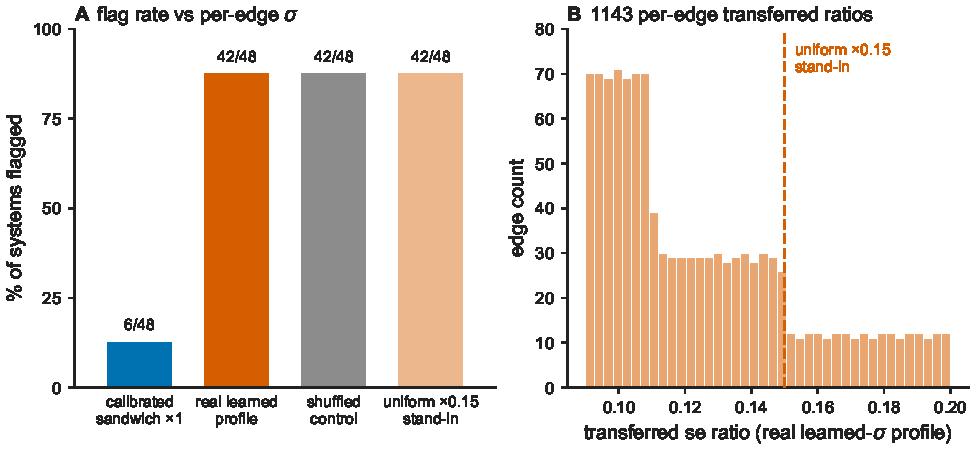
\includegraphics[width=\textwidth]{figP4_sigma_profile.pdf}
\caption{\textbf{Cycle-closure flagging under four per-edge $\sigma$ assignments, and the
distribution of the real-profile ratios.} (Left) Percentage of the $48$-system OpenFE
network flagged, for the calibrated sandwich, the learned head's measured overlap-dependent
miscalibration profile transferred by percentile rank onto each edge's own overlap, a
shuffled-profile control, and a uniform $\times0.15$ shrink. (Right) Histogram of the $1143$
per-edge transferred ratios from the real learned profile, with the uniform $\times0.15$
stand-in marked.}
\label{fig:P4}
\end{figure}

\paragraph{Dose-response of the QC to $\sigma$ miscalibration (Figure~\ref{fig:P4b}).}
Figure~\ref{fig:L}B and Supplementary Figure~\ref{fig:P4} each characterize the closure test
at a small number of scale points (${\times}1$ calibrated, ${\times}0.15$ stress test / real
profile); here a pre-registered, frozen grid of $16$ uniform $\mathrm{se}$ scale factors
($2.0$--$0.10\times$) is swept through the identical GLS $+$ Benjamini--Hochberg pipeline on the
same $48$-system OpenFE network. Two readouts were frozen in advance: $s_{\text{onset}}$, the
largest scale that flags strictly more systems than calibrated, and $s_{50}$, the largest scale at
which at least half the systems are flagged. $s_{\text{onset}}=0.9\times$ ($7/48$ vs.\ the calibrated $6/48$) is exactly
one system crossing the Benjamini--Hochberg threshold. That readout is grid-determined rather than
a measurement of this benchmark: because the flagged count is monotone in the scale, a
strictly-exceeds-calibrated onset returns whichever grid point below $1.0$ sits just past the first
system's threshold crossing. Independent probing places that system's crossing as high as
$s=0.995\times$, so a finer grid would return $s_{\text{onset}}=0.995\times$, and in the continuum
limit $s_{\text{onset}}\to1.0\times$ for any benchmark with a system near the cutoff. It is
reported as the pre-registered readout. The informative readout is magnitude-based, such as the
largest scale that doubles the calibrated count, which here is $0.7\times$ at $12/48$. The
substantive change is mid-curve: from $0.7\times$ to $0.3\times$ the flagged fraction climbs from $12/48$
($25\%$) to $30/48$ ($62\%$), reaching half the benchmark at $s_{50}=0.3\times$ (the true $50\%$
crossing is bracketed by the adjacent $0.35\times$ and $0.30\times$ grid points, which flag
$23/48$ and $30/48$ respectively). The learned head's measured, rank-transferred miscalibration
band ($0.09$--$0.20\times$; Figure~\ref{fig:Afoils}, Supplementary Figure~\ref{fig:P4}) lies entirely
below $s_{50}$, so the head is not near the transition but well inside the saturated regime. The
over-wide half of the grid is not flat either: relative to the calibrated $6/48$, a bar
only $30\%$ too wide ($1.3\times$) already loses five of the six flagged systems ($1/48$), and any
wider bar ($1.5\times$, $2.0\times$) flags none, so the requirement is calibration, not
conservatism. Two consistency
checks confirm that the sweep reproduces the published test path: the ${\times}1.0$ row reads
$6/48$, matching Figure~\ref{fig:L}A's calibrated count, and the ${\times}0.15$ row reads $42/48$,
matching Figure~\ref{fig:L}B and Supplementary Figure~\ref{fig:P4}'s uniform/real-profile arms.
The response to the shrink magnitude is graded rather than
threshold-like. The closure test is therefore selective over roughly a factor of three of
$\sigma$ under-estimation below the calibrated scale, and over-wide $\sigma$ costs power in the
other direction, so the calibrated scale is a two-sided optimum rather than a plateau. The sweep is deterministic: the sixteen scale factors are a frozen
grid and the test at each of them is a closed-form recomputation on fixed inputs, so re-running
reproduces the entire curve exactly.

\begin{figure}[t]\centering
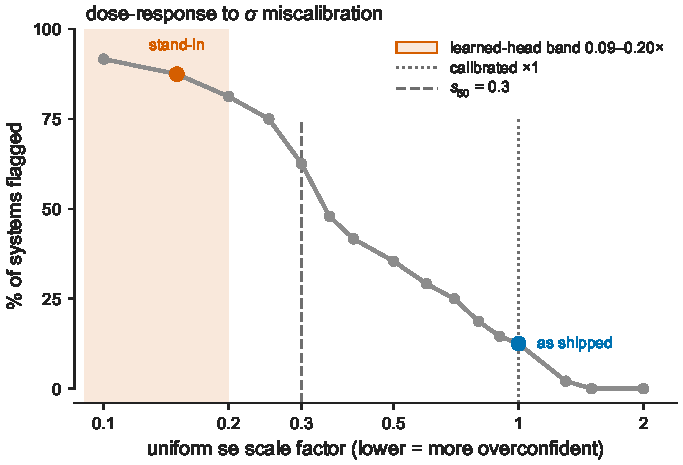
\includegraphics[width=0.7\textwidth]{figP4b_dose_response.pdf}
\caption{\textbf{Fraction of the OpenFE network flagged across a swept uniform $\sigma$ scale
factor.} Percentage of the $48$-system network flagged by the cycle-closure test, across a
frozen grid of $16$ uniform standard-error scale factors from $2.0\times$ to $0.10\times$
(lower $=$ more overconfident; $1.0\times$ is the calibrated sandwich). Vertical dotted
line: the calibrated scale. Vertical dashed line: $s_{50}$, the largest scale at which at
least half the systems are flagged. Shaded band: the learned head's measured,
rank-transferred miscalibration range.}
\label{fig:P4b}
\end{figure}

\paragraph{Per-system flag robustness to each system's own calibration error (Table~\ref{tab:P8}).}
The Figure~\ref{fig:L} flag set raises a mild circularity concern: the per-system calibration of
the sandwich null, measured independently against across-replicate spread
(Figure~\ref{fig:Arep}), is heterogeneous, and four of the six flagged systems are themselves
locally overconfident (\texttt{brd4} $0.76\times$, \texttt{faah} $0.90\times$, \texttt{bace}
$0.96\times$, \texttt{hif2a} $0.96\times$; only \texttt{cdk8} $1.41\times$ and \texttt{p38}
$1.43\times$ are conservative), so a flag could partly reflect that system's own too-tight bars
rather than genuine physical inconsistency. That concern is tested directly. For replicate $0$, over the $48$
systems with $\geq1$ independent cycle (the identical population as Figure~\ref{fig:L}), each
system's per-edge $\mathrm{se}$ is inflated by $1/\mathrm{ratio}$ where its own ratio is below
$1$ (systems with ratio $\geq1$ are already conservative and are left unchanged), and the
Benjamini--Hochberg test is recomputed over the whole set under this self-calibrated null.
The criterion was fixed in advance: the result stands if every nominally-flagged system remains flagged, and is partial or negative if only some or none do. The population, the inflation rule and $\alpha=0.05$ were fixed
before this run. All six flags remain under their own self-calibrated null (Table~\ref{tab:P8}), each self-calibrated reduced $\chi^2$
($2.36$--$8.97$) remaining far above the level a sampling-consistent network of this size and
degree-of-freedom profile shows (Section~\ref{sec:qc}, main text). This check pools the ratio over
a whole system; the same one-sided inflation applied at the per-edge granularity this work
pre-specified retains two of the six, and Table~\ref{tab:selfgrid} reports both granularities in
both directions. The distribution-free
cross-replicate reproduction check of Figure~\ref{fig:Lval}B is a function of raw residual
correlation only, never of $\mathrm{se}$, so it does not depend on this null and is not affected
by this concern in either direction. The per-system ratio in Table~\ref{tab:P8} is the
root-mean-square reported standard error over the root-mean-square across-independent-replicate
SD, pooled per system, not a naive per-system average of per-edge ratios or a naive ratio of
arithmetic means, which for three of the six systems below would sit on the opposite side of
$\mathrm{ratio}=1$. The ratios are raw $n{=}3$ SD ratios. Their residual small-sample bias is
upward and target-specific, of order the reciprocal of the edge count, so debiasing would move all
four of the locally overconfident flagged systems (\texttt{brd4} $0.76\times$, \texttt{faah}
$0.90\times$, \texttt{bace} and \texttt{hif2a} $0.96\times$) further below one rather than toward
it; the raw ratios used here are generous to those systems rather than the reverse. The computation
is deterministic, and the full $48$-system table is released with the analysis code.

\begin{table}[t]\centering
\caption{\textbf{Per-system reduced $\chi^2$ before and after inflating each system's own
per-edge standard error by its own measured calibration error.} ``ratio'' is the per-system
root-mean-square ratio of reported standard error to across-replicate standard deviation of
binding $\ddG$, at $n=3$. $\chi^2_{\text{nom}}$ is the nominal reduced $\chi^2$;
$\chi^2_{\text{self}}$ inflates that system's own standard error by $1/\mathrm{ratio}$ where
$\mathrm{ratio}<1$ and leaves it unchanged otherwise. Rows are the six flagged systems.}
\label{tab:P8}
\small
\begin{tabular}{@{}lrrrl@{}}
\toprule
System & ratio & $\chi^2_{\text{nom}}$ & $\chi^2_{\text{self}}$ & Still flagged \\
\midrule
\texttt{brd4}  & $0.76$ & $15.40$ & $8.97$ & yes \\
\texttt{bace}  & $0.96$ & $5.57$  & $5.13$ & yes \\
\texttt{faah}  & $0.90$ & $3.71$  & $2.99$ & yes \\
\texttt{cdk8}  & $1.41$ & $2.68$  & $2.68$ & yes (unchanged; already conservative) \\
\texttt{hif2a} & $0.96$ & $2.53$  & $2.36$ & yes \\
\texttt{p38}   & $1.43$ & $2.40$  & $2.40$ & yes (unchanged; already conservative) \\
\bottomrule
\end{tabular}
\end{table}

\paragraph{The downstream audit: what is under test (Table~\ref{tab:audit}).} The test of
Section~\ref{sec:qc} runs on a network's own residuals. Whether the same free calibration also
improves downstream machine learning is a separate question, and the six tasks collected in
Table~\ref{tab:audit} are the audit of it. Three performance tasks, interval sharpness,
commit-to-synthesis selection and reward re-ranking over a measured congeneric set, run with the
commit-trust decision task on the public OpenFF protein--ligand
benchmark~\citep{hahn2022plbench} (FEP+ and Merck data~\citep{wang2015fep,schindler2020merck},
experimental $\ddG$ labels, both-endpoint scaffold-disjoint out-of-distribution splits); edge
ranking in active learning and the stopping decision run in controlled simulations. The amortized
$\sigma$ under test is the predictive uncertainty of the amortized $\ddG$ predictor, the trunk
specified above, on unseen $\ddG$,
$\sigma_{\text{total}}=\gamma\sqrt{\sigma^2_{\text{ens}}+\sigma^2_{\text{ale}}}$: deep-ensemble
epistemic spread and benchmark aleatoric floor, conformally scaled at miscoverage $\alpha=0.1$. It
is \emph{not} the per-edge BAR sampling standard error of Figure~\ref{fig:A} or its
learned-variance baseline of Figure~\ref{fig:Afoils}; a bare ``$\sigma$'' anywhere in this audit
means $\sigma_{\text{total}}$.

\paragraph{Sharpness, ranking and selection (Figures~\ref{fig:Breal} and~\ref{fig:J}A).} On real
held-out residuals of that trunk at matched $\sim$$0.90$ marginal coverage the decomposed interval
is slightly wider than flat split-conformal (width ratio $0.92\times$), because epistemic spread is
small against the large irreducible out-of-distribution error; its conditional calibration is
comparable to a fair Mondrian-by-target conformal and the advantage is not significant
(ours$-$split $-0.044$ $[-0.121,0.005]$). The synthetic illustration above, whose generative
structure the decomposition knows, is up to $2.2\times$ sharper than split-conformal; that does not
transfer. For edge ranking, sandwich against naive weights differ by $0.98\times$ $[0.93,1.03]$ on
calls-to-top-$k$ (above): in a connected graph the GLS contrast mean is unbiased for any positive
weights, so the weight value is second-order for ranking. So too for commit selection at matched volume,
where the $\sigma$-aware ranking does not beat a raw-$\mu$ ranking ($-0.006$ $[-0.016,0.007]$). A
calibrated bar informs whether to act and not which action ranks first.

\paragraph{Commit trust against recalibrated baselines (Figure~\ref{fig:J}B).} Fixing the ensemble
mean and varying only the uncertainty in a commit rule (commit iff the lower-confidence bound
$\mu-\kappa\sigma\ge\tau$), an overconfident epistemic-only $\sigma$ over-claims badly: its
realized-versus-claimed correctness shortfall is $+0.182$ $[0.132,0.225]$ larger than the
decomposed $\sigma$'s. That number quantifies miscalibration; it does not rank the ways of curing
it. On the same scale, temperature scaling~\citep{guo2017calibration} of that overconfident $\sigma$
leaves $+0.034$ $[-0.018,0.081]$. Split-conformal recalibration of it leaves $-0.029$
$[-0.077,0.007]$. Both straddle zero, in opposite directions. Trustworthy decisions need calibration, and all three
routes supply it. Neither does this task separate them on
cost, since all three fit a scalar on the same held-out split; the closed form's cost advantage is
the one Section~\ref{sec:bar} measures, a per-edge variance computed rather than learned, and none
of these six tasks tests it.

\paragraph{Reward re-ranking over a measured congeneric set (Figure~\ref{fig:K}).} Driving a
trajectory-balance GFlowNet~\citep{bengio2021gflownet,malkin2022tb} over \texttt{eg5} (the most
$\sigma$-varying evaluable target), the
calibrated lower-confidence-bound (LCB) reward lowers the true hit-rate, $0.140$ against a raw
predicted-mean reward's $0.249$ (cal$-$raw $-0.109$),
because on this set $\sigma$ tracks chemical novelty
($\mathrm{corr}(\sigma_{\text{total}},\text{affinity})=+0.42$) rather than low quality. An LCB
reward improves the hit-rate only where $\sigma$ flags low-quality candidates
(Table~\ref{tab:audit} below).

\begin{figure}[t]\centering
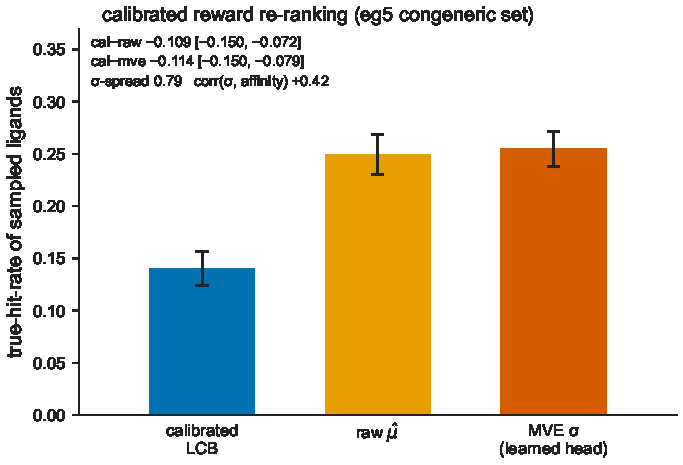
\includegraphics[width=0.7\textwidth]{figK_calibrated_generation.pdf}
\caption{\textbf{True hit-rate of a trajectory-balance GFlowNet under three reward
functions.} Mean true hit-rate of generated ligands, over $12$ seeds with standard-error
bars, for a calibrated lower-confidence-bound reward, a raw predicted-mean reward, and
an overconfident MVE-uncertainty reward, on the \texttt{eg5} congeneric ligand series.}
\label{fig:K}
\end{figure}

\begin{figure}[t]\centering
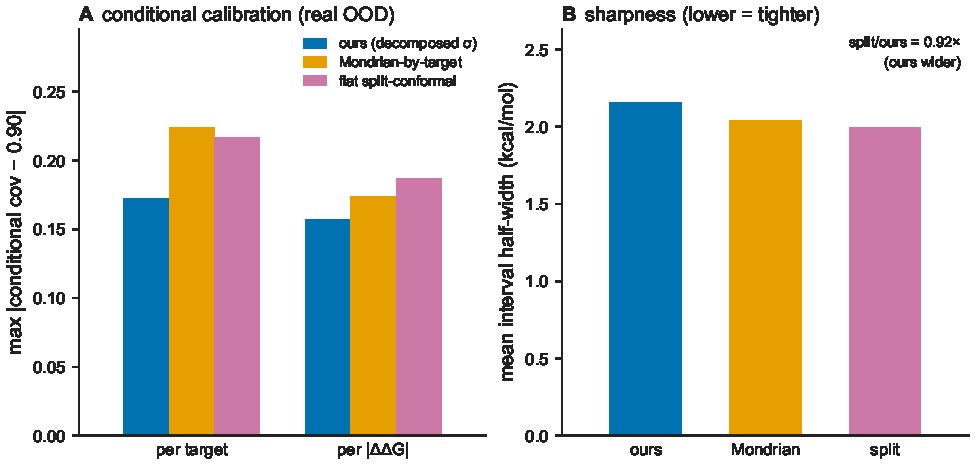
\includegraphics[width=\textwidth]{figB_real_decomposition.pdf}
\caption{\textbf{Conditional calibration and interval sharpness on real out-of-distribution
trunk residuals.} (A) Maximum conditional coverage error, computed per target and per
$|\ddG|$ bin, for the decomposed physics $\sigma$, a Mondrian-by-target conformal interval,
and a flat split-conformal interval, each at approximately $90\%$ marginal coverage.
(B) Mean prediction-interval half-width for the same three methods.}
\label{fig:Breal}
\end{figure}

\begin{figure}[t]\centering
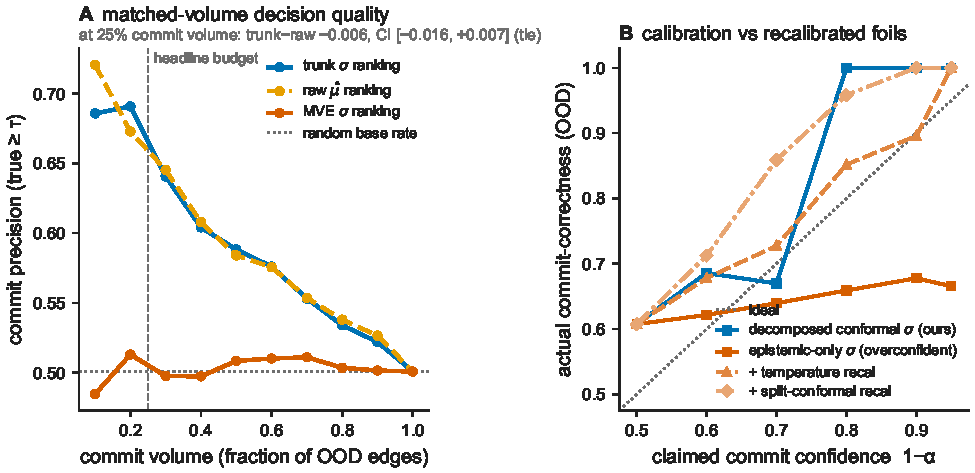
\includegraphics[width=\textwidth]{figJ_amortized_reward.pdf}
\caption{\textbf{Commit-to-synthesis ranking and calibration on real out-of-distribution
edges.} (A) Commit precision (fraction of committed candidates with true value at or above a
threshold $\tau$) versus commit volume (fraction of edges committed), for candidates ranked
by the trunk $\sigma$-aware margin, by the raw predicted mean, and by a learned MVE-head
margin, with the random base rate marked. (B) Actual commit-correctness versus claimed
commit confidence $1-\alpha$, for the decomposed physics $\sigma$, an epistemic-only
$\sigma$, and the same epistemic-only $\sigma$ after temperature and after split-conformal
recalibration, with the ideal (actual = claimed) line.}
\label{fig:J}
\end{figure}

\begin{figure}[t]\centering
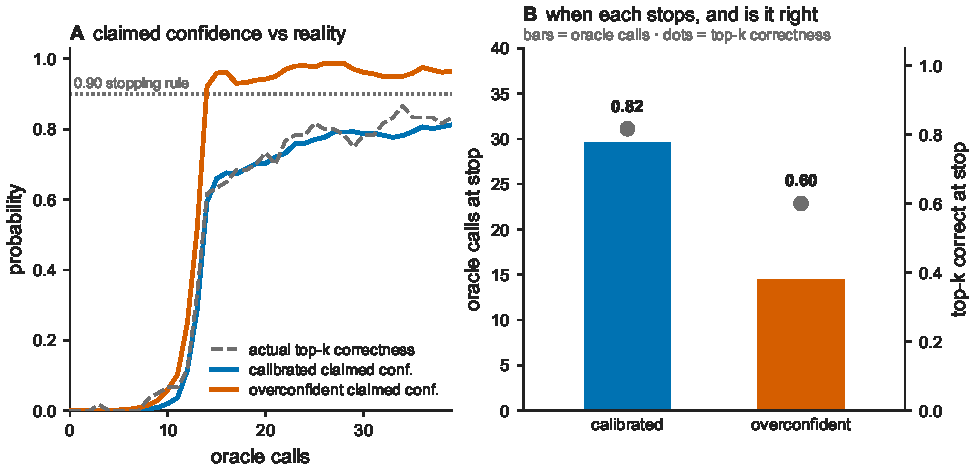
\includegraphics[width=\textwidth]{figG_calibrated_stopping.pdf}
\caption{\textbf{Simulated active-learning stopping under calibrated versus counterfactually
overconfident claimed uncertainty.} (A) Actual top-$k$ correctness and claimed stopping
confidence, averaged over $60$ seeds, versus the number of oracle calls, for a calibrated
learner and for a learner whose assumed posterior standard error is scaled by $0.15\times$.
(B) Oracle calls at the stopping rule (bars) and top-$k$ correctness at
that stop (points), for the two learners.}
\label{fig:G}
\end{figure}

\paragraph{The stopping decision as a function of the assumed error
(Table~\ref{tab:gsweep}).} Figure~\ref{fig:G} reports one point of a curve. The experiment
measures how the stopping decision depends on the error the learner assumes, everything else
held fixed, and the whole dependence is tabulated here. The $0.15\times$ arm of
Figure~\ref{fig:G} is a counterfactual stand-in: it imposes on the assumed error the
miscalibration measured for a trained per-edge head in Figure~\ref{fig:Afoils}, and is not an
estimator run here. The two arms of the figure keep their own Monte-Carlo stream, so adding
the sweep points leaves them unchanged.

\begin{table}[t]\centering
\caption{\textbf{Simulated stopping under a swept assumed error.} Assumed posterior standard
error as a multiple of the true one, against oracle calls at the stopping rule, top-$k$
correctness at that stop, and the mean absolute gap between claimed confidence and actual
correctness over the budget; $60$ seeds. Starred rows are the two arms of
Figure~\ref{fig:G}.}
\label{tab:gsweep}
\small
\begin{tabular}{@{}lrrr@{}}
\toprule
assumed se / true se & calls at stop & correct at stop & mean $|$claimed $-$ actual$|$ \\
\midrule
$1.06\times$ (conservative)      & $30.8$ & $0.83$ & $0.027$ \\
$1.00\times$ (calibrated)$^{*}$  & $29.6$ & $0.82$ & $0.022$ \\
$0.94\times$                     & $28.4$ & $0.82$ & $0.020$ \\
$0.80\times$                     & $25.4$ & $0.82$ & $0.029$ \\
$0.60\times$                     & $21.1$ & $0.77$ & $0.059$ \\
$0.40\times$                     & $17.9$ & $0.68$ & $0.093$ \\
$0.20\times$                     & $14.9$ & $0.60$ & $0.127$ \\
$0.15\times$ (stand-in)$^{*}$    & $14.4$ & $0.60$ & $0.137$ \\
\bottomrule
\end{tabular}
\end{table}

The $0.94\times$ row is the $6\%$ under-estimate a same-budget estimator pooling single-label
edges by overlap reaches on the identical labels the heads were given (Figure~\ref{fig:Afoils}).
At that scale the stopping decision is indistinguishable from the calibrated one, $28.4$
calls against $29.6$ at the same $0.82$ correctness. Correctness at the stop first moves at
$0.60\times$, and the halved budget of Figure~\ref{fig:G}B needs $0.20\times$. The contrast
is therefore scoped, exactly as the quality-control collapse of the main text is scoped, to
per-edge heads missing by $5$--$11\times$, and is not evidence that a same-budget learned
estimator would stop early. The one effect that survives a fair comparison is in the opposite
direction: a $6\%$ over-estimate spends $30.8$ calls for the same correctness, the decision cost of
a conservative bar of Figure~\ref{fig:J}B.

\paragraph{The decision cost of a conservative bar (Figure~\ref{fig:J}B).}
Even a conservative bar carries a decision cost: a systematic
${\sim}1.41\times$ se inflation is itself a (safe-direction) miscalibration that, via
the LCB rule, biases toward late stopping and under-commit. It errs in the safe direction against
sampling noise, and because the independent-replicate SD is itself a lower bound
on full reproducibility (Section~\ref{sec:bar}), the inflation may be
closer to neutral against the true run-to-run spread once pose and system-preparation variance
are included.

\paragraph{Downstream audit summary (Table~\ref{tab:audit}).} Table~\ref{tab:audit} collects,
for four downstream performance tasks (interval sharpness, active-learning edge weighting,
commit-to-synthesis ranking, and reward re-ranking on the \texttt{eg5} congeneric set) and two
decision tasks (commit trust and active-learning stopping), the calibrated method's effect
relative to the relevant baseline. The top block shows no measurable performance gain
(Figures~\ref{fig:Breal}, \ref{fig:C}, \ref{fig:J}A, \ref{fig:K} above). The bottom block
shows what the two decision tasks are measured against: an overconfident $\sigma$ and a
counterfactual stand-in are both far worse, which measures the cost of miscalibration, while against a fair
baseline, the same overconfident $\sigma$ after temperature or split-conformal
recalibration and a same-budget pooled estimator at its measured $0.94\times$, the effect is
absent (Figures~\ref{fig:J}B, \ref{fig:G} and Table~\ref{tab:gsweep} above).

\begin{table}[t]\centering
\caption{\textbf{Effect of the decomposed $\sigma$ relative to a baseline, across six
downstream tasks.} Effects are the calibrated method minus the relevant baseline with a
$95\%$ bootstrap confidence interval; ``real'' denotes OpenFF benchmark out-of-distribution
edges, ``sim'' denotes a controlled simulation. The two decision tasks are each given against
an uncalibrated foil and against a fair baseline: the same $\sigma$ recalibrated, and the
assumed error a same-budget pooled estimator reaches.}
\label{tab:audit}
\small
\begin{tabular}{@{}p{3.1cm}lp{5.4cm}p{2.6cm}@{}}
\toprule
Downstream task & Data & Effect (calibrated $-$ baseline) [95\% CI] & Verdict \\
\midrule
Interval sharpness (out-of-distribution) & real & width split/decomposed $0.92\times$; cond.\ $-0.044$ $[-0.121,0.005]$ & no gain \\
Edge weighting (active learning) & sim & calls-to-top-$k$ $0.98\times$ $[0.93,1.03]$ & no gain \\
Commit ranking (matched volume) & real & precision $-0.006$ $[-0.016,+0.007]$ & tie \\
Reward re-ranking (evaluable set, \texttt{eg5}) & real & true hit-rate $-0.109$ $[-0.150,-0.072]$ & hurts (directional, single target)$^{a}$ \\
\midrule
Commit trust vs overconfident $\sigma$ & real & shortfall $+0.182$ $[0.132,0.225]$ better & cost of miscalibration \\
Commit trust vs temperature-scaled $\sigma$ & real & shortfall $+0.034$ $[-0.018,+0.081]$ & tie \\
Commit trust vs split-conformal $\sigma$ & real & shortfall $-0.029$ $[-0.077,+0.007]$ & tie \\
Stopping vs $0.15\times$ stand-in & sim & $82\%$ vs $60\%$ correct at stop & cost of miscalibration \\
Stopping vs pooled estimator ($0.94\times$) & sim & $0.82$ vs $0.82$ correct, $29.6$ vs $28.4$ calls & tie \\
\bottomrule
\end{tabular}

\smallskip
\noindent{\footnotesize $^{a}$The reward re-ranking effect is measured on a single evaluable
target (\texttt{eg5}) and is directional, and it is not yet established as a general
property of calibrated reward re-ranking across chemotypes.\par}
\end{table}


\paragraph{What the audit establishes.} None of the six tasks puts the calibrated $\sigma$ ahead of
a fair baseline. On commit trust the physics $\sigma$ matches post-hoc recalibration rather than
beating it, and the stopping separation is absent at the six per cent a same-budget pooled
estimator produces. The audit establishes a precondition rather than an advantage: decisions of
this kind need calibration, an overconfident $\sigma$ corrupts them, and the calibration
demonstrably helps on real data inside the network, as the null of the test of
Section~\ref{sec:qc}, rather than downstream of it. The graph weight contributes the same
way, through structure rather than magnitude, making the gauge directions exactly unidentifiable
(Theorem~\ref{thm:fr}) while by Gauss--Markov its value does not improve ranking.

\paragraph{Provenance of the experimental affinities.} The grounding against measured affinity
uses one ChEMBL target per system, verified to be a human single-protein target before use, and
one assay type per system, taken in the order $\mathrm{IC}_{50}$ then $K_i$ and never mixed within
a system. A flagged system enters the guided-versus-random comparison only if at least $60\%$ of
its network ligands map to a measured value. The counts here are grounded ligands, which for two
systems exceed the ligand count of the sub-network the measurement runs on by one: an edge enters
only when both its endpoints carry an affinity, so a ligand all of whose partners are ungrounded
drops out. That is \texttt{1\_1W7H} on \texttt{p38} ($35$ grounded, $34$ in the sub-network) and
\texttt{CAT-4j} on \texttt{bace} ($24$ and $23$); \texttt{cdk8} and \texttt{hif2a} lose none. The \texttt{eg5} grounding of Section~\ref{sec:qc}
predates that coverage-gated join and was assembled differently, per ligand from one named ChEMBL
assay rather than by a target-wide structure search, so its row records the assay as well as the
target. Table~\ref{tab:chembl} lists what was used.

\begin{table}[t]\centering
\caption{\textbf{ChEMBL provenance of the experimental affinities.} Target identifier, protein,
assay type, and the number of network ligands with a measured value, for every system grounded
against measured affinity: the four flagged systems that clear the $60\%$ coverage requirement,
and \texttt{eg5}, the clean system used for the comparison of accuracy against experiment. Affinities are converted at $RT\ln 10 = 1.364$ kcal/mol and
aggregated per ligand by the median pChEMBL value.}
\label{tab:chembl}
\small
\begin{tabular}{@{}llll r@{}}
\toprule
system & ChEMBL target & protein & assay & ligands \\
\midrule
\texttt{cdk8}  & CHEMBL5719    & cyclin-dependent kinase 8    & $\mathrm{IC}_{50}$ & $24$ \\
\texttt{hif2a} & CHEMBL1744522 & endothelial PAS domain protein 1 & $\mathrm{IC}_{50}$ & $41$ \\
\texttt{p38}   & CHEMBL260     & mitogen-activated protein kinase 14 & $\mathrm{IC}_{50}$ & $35$ \\
\texttt{bace}  & CHEMBL4822    & beta-secretase 1             & $\mathrm{IC}_{50}$ & $24$ \\
\midrule
\texttt{eg5}   & CHEMBL4581    & kinesin-like protein KIF11   & $\mathrm{IC}_{50}$ & $28$ \\
\bottomrule
\end{tabular}

\smallskip
\noindent{\footnotesize The \texttt{eg5} affinities were taken from a single named ChEMBL ATPase
$\mathrm{IC}_{50}$ assay, identifier CHEMBL1101849, queried per ligand; the other four rows come
from a target-wide connectivity-based structure search under the $60\%$ coverage rule, for which
no single assay identifier applies.\par}
\end{table}


\bibliographystyle{plainnat}
\bibliography{refs}
\end{document}
